% The prose of results/f49f6c7d-pherc0826-chain, written as LaTeX from the start: this work has no
% draft.md, so nothing converts into this file and nothing here is generated. Every number is a
% macro of numbers.tex, written by src/tools/paper_numbers.py. A paragraph that uses a macro whose
% file does not exist yet sits between a PENDING-BEGIN and a PENDING-END line: the build refuses the
% article while any such macro is undefined, and only its preview mode drops those paragraphs.
%
% Scope, director 2026-09-28T08:03:17Z (owner's rule): the article measures only the assembly, all on
% PHerc. 0826, with item 91 as its comparison. Each component work is cited for what its module is and
% for its measured change on its author's own data. Stevens' 365 cm2 on PHerc. 1667 appears only as a
% labelled reference on another scroll. Nothing here is a reading of ink.
%
% Lean pass of 2026-09-30 (director's brief, owner's word): one short section for Stevens' stages, a
% results section of its own for the checks and the certified square, open questions and a conclusion,
% the appendix after the references (appendix.tex). Locations on the scroll are withheld. Our upstream
% items are cited only when open or merged.

\maketitle

\begin{abstract}
The organisers of the Vesuvius Challenge ask how to make the reading of a scroll work ``automatically, reliably, and
at scale for every scroll'', and among its bottlenecks they name a traced sheet that jumps from one wrap to another,
for which they want ``Smarter surface tracing algorithms that avoid introducing sheet switches''~\cite{openproblems}.
We built a loop that runs Stevens' published pipeline~\cite{stevenssr} on the unread PHerc.~0826 with no person in it,
chooses where each surface starts, and keeps a surface only where a set of automatic checks finds no fault. A square is certified when none of its cells is a hole,
crosses one of the sheets it is compared with, folds onto the next winding or lies in a cluster of points that run
steeply across the surface prediction. Where two traced surfaces cross, the one our sheets agree with less loses the
cell. On a surface grown by the organisers' tracer from a
start our search chose, the checks certify a square of \RcOneSquare{}~mm on one lamina. They also reject the
\FibreTopFailCount{} largest certified pieces of our own sheets, which fail a fibre test. Our faster bad patch finder
and growth build together make Stevens' pipeline \ArmFactorAC{} times faster per seed with every measured output
equal, the growth build alone \ArmFactorBC{}; the chain as delivered also carries \CorrOutput{} corrections that change
its sheets. The checks
establish geometry, not legibility. On labelled PHerc.~0139 our sheets carry the ink to the released model, but our label
free statistic does not see that ink, so no reading of PHerc.~0826 is claimed.
\end{abstract}

\begin{figure*}[!t]
\centering
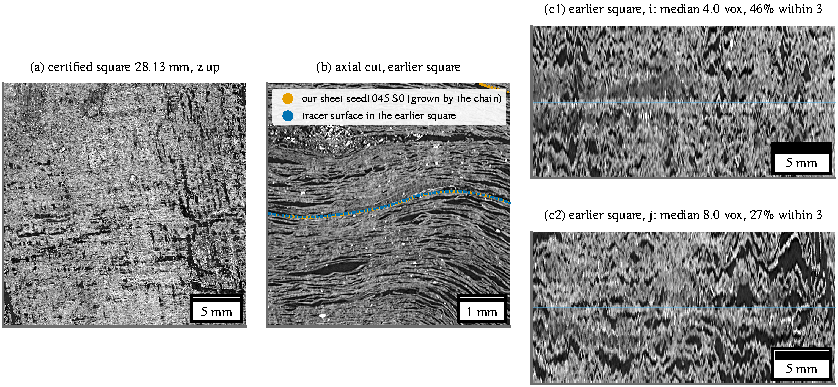
\includegraphics[width=\textwidth]{figures/c-f21-r2c}
\caption{\CaptionRtwoC}
\label{fig:r2c}
\end{figure*}

\begin{figure*}[p]
\centering
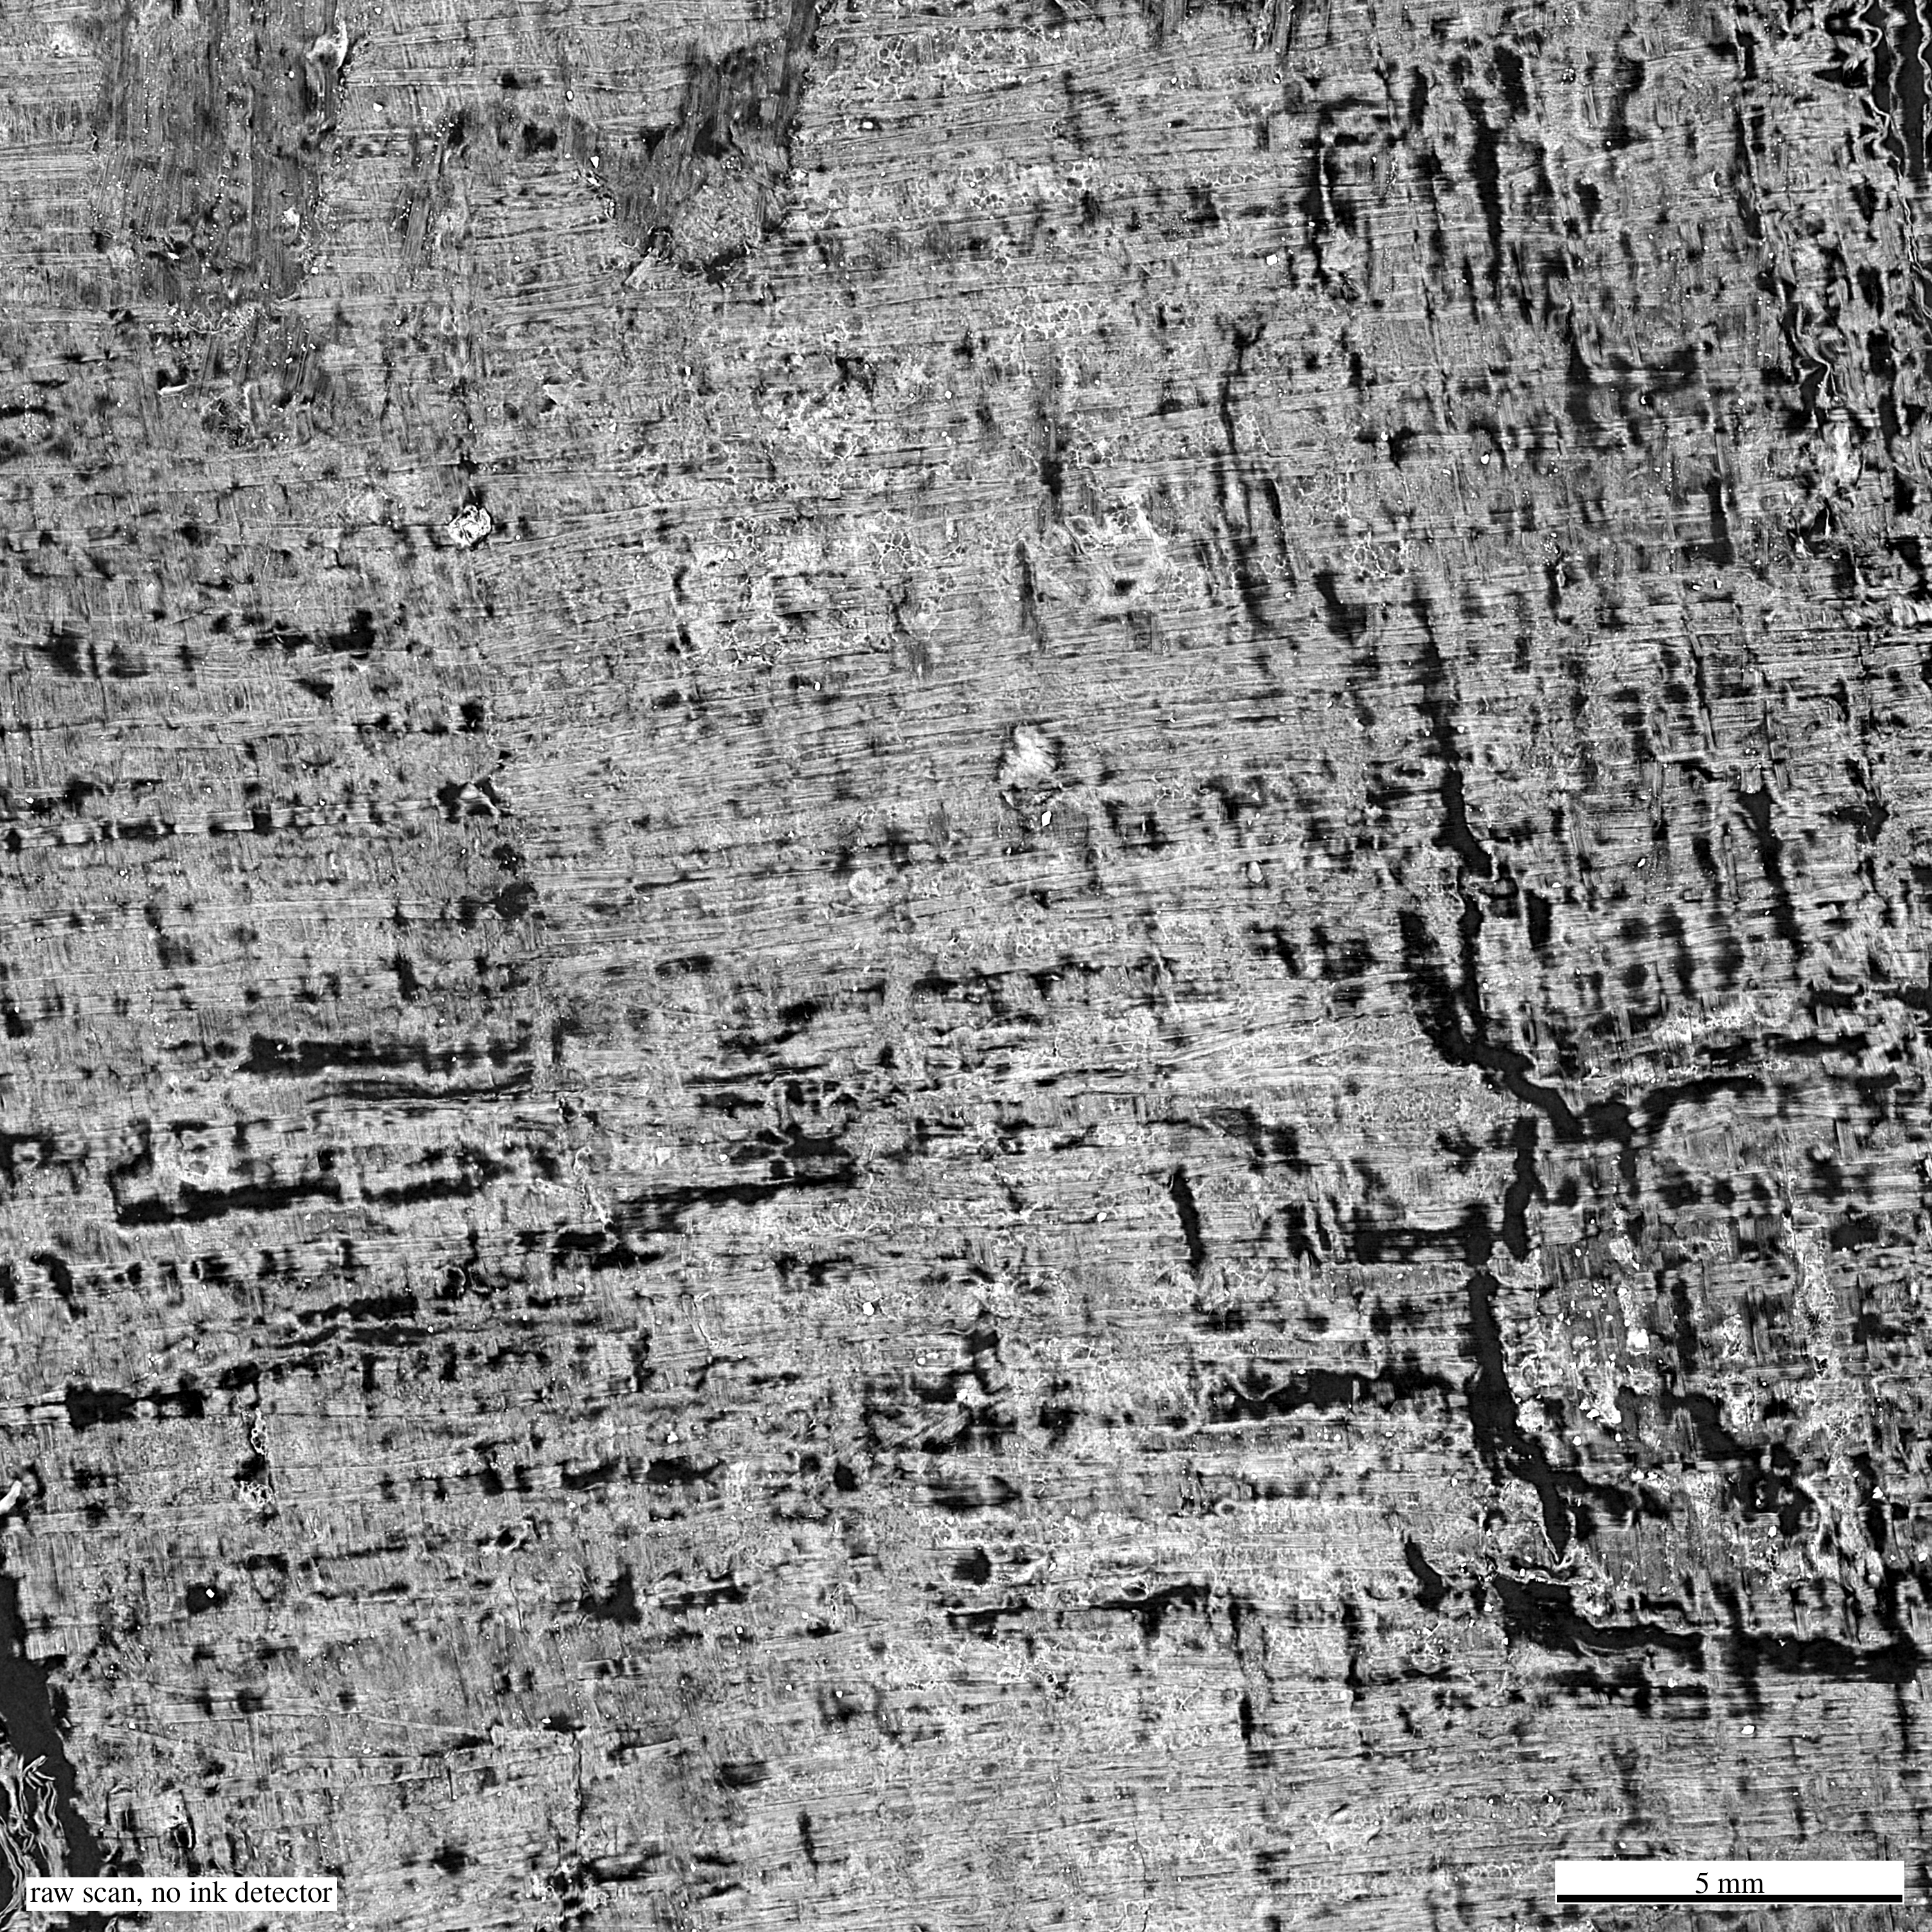
\includegraphics[width=\textwidth]{figures/c-f25-square-full}
\caption{\CaptionSquareFull}
\label{fig:squarefull}
\end{figure*}

\begin{figure*}[t]
\centering
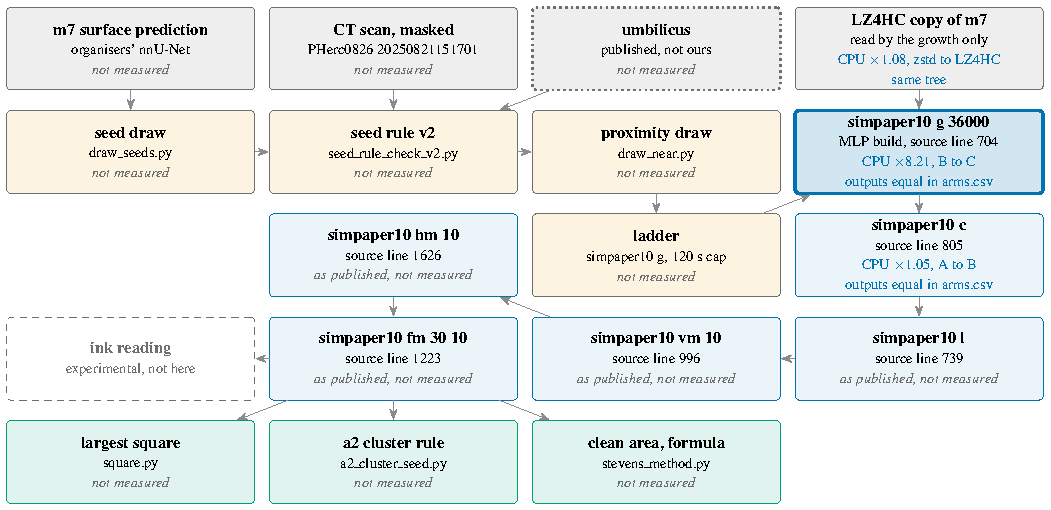
\includegraphics[width=\textwidth]{figures/c-f1-pipeline}
\caption{The pipeline run on PHerc.~0826, each box the program and mode it runs. The third line of a
box is the factor by which our change made that step faster, the earlier median CPU time over the
later on the same seeds. It comes from the arms of Section~\ref{sec:arms} or, for the LZ4HC copy, the quiet
clocks of Section~\ref{sec:growth}. On the growth and the bad patch finder it also says whether the two
arms compared are equal on every output column of \texttt{arms.csv}: the median sheets, formula area, square, a2 share, crossing cells
and deaths. That is equality of those measures, not byte identity of the sheets. The LZ4HC copy's
«same tree» is the byte identity test of Section~\ref{sec:inputs}. A box with no measured factor says
so. Grey:
the inputs; orange: the seed selection; blue: Stevens' program \texttt{simpaper10}, with the line of
each mode in his published source (commit \SrCommit{}); green: the measures of each delivered sheet;
dashed: a reading of ink, which is experimental and not part of this article. Drawn from
\texttt{src/evidence/figures/c-f1-pipeline.csv}.}
\label{fig:pipeline}
\end{figure*}

\section{Introduction}
\label{sec:intro}

The organisers of the Vesuvius Challenge state the open problem plainly: ``The harder question is how to make the same
process work automatically, reliably, and at scale for every scroll''~\cite{openproblems}. Among the bottlenecks they
list, a traced sheet can switch layers (``Meshes can jump from one wrap to another''), and what they ask for is
``Smarter surface tracing algorithms that avoid introducing sheet switches''. They also ask whether the whole workflow can be made
``reproducible enough for collection-scale reading''. This article answers a narrow part of that question on one scroll
that is still unread.

The engine is not ours. The scan of PHerc.~0826, its surface prediction (the m7 nnU-Net output) and its umbilicus are
published by the organisers~\cite{opendata}. The growth that fits small patches of surface to that prediction, and the
four stages that join the patches and flatten them into sheets, are Stevens' program \texttt{simpaper10}~\cite{stevenssr},
which the arms of Section~\ref{sec:arms} run as he published it except for how it is built and a faster bad patch
finder. The chain that delivered this article's sheets also carries \CorrOutput{} corrections of his source that change
what is grown, and \CorrInert{} that do not (Section~\ref{sec:growth}). The surface tracer that grows the surface of this
article's headline square, \texttt{vc\_grow\_seg\_from\_seed} of \texttt{villa} run on the normal grids of
\texttt{vc\_gen\_normalgrids}~\cite{villa}, is theirs, and so is the renderer that turns a surface into the layers an ink
model reads. The ink model is the one the organisers released~\cite{inkmodel}; we report its reads only on a labelled
control scroll.

What is ours is the loop around the engine and the checks that judge its output, and Figure~\ref{fig:pipeline} names
every program and mode the loop runs. The loop picks seeds that avoid the solid blocks of the surface prediction. Our faster
bad patch finder and growth build together make Stevens' pipeline \ArmFactorAC{} times faster in median CPU time per
seed, the growth build alone \ArmFactorBC{}, with every output column of the arms table equal (Section~\ref{sec:arms}).
The chain grows its seeds with that build plus the corrections, whose sheets differ (Section~\ref{sec:growth}). The checks decide without a person which surface to
keep (Section~\ref{sec:checks}). A crossing map finds where two sheets cross, the a2 rule finds a sheet that runs
steeply across the prediction, and a one lamina test finds a sheet folded onto the next winding. In this article a
square or a piece of a sheet is certified, or certified on one lamina, when it has no hole and no cell that fails a
check, as our certification tool computes it. A cell fails when it crosses one of the \UnionSheets{} sheets delivered
for the \AreaSeeds{} seeds of the area study (Section~\ref{sec:out}) or another sheet of its own seed, when the one
lamina test flags it because the same surface lies about one pitch away along its normal, or when it lies in a cluster
of steep points that the a2 cluster rule cuts out; a steep point outside such a cluster does not fail its cell. A
surface grown by the organisers' tracer is compared with the same \UnionSheets{} sheets and with the tracer's other
surfaces, and a cell where two traced surfaces cross fails for the one that agrees less with our sheets there, and for
both when they agree equally. The words mean these checks passed and nothing more. A fibre score of the raw scan and a search for clean
windows of \WinArea{}~cm$^2$ complete the checks. These checks are how the loop chooses which surface to
keep, whichever program grew it. They do not make a tracer avoid a switch; they keep a surface only where they see none.
On PHerc.~0826 they certify a square of \RcOneSquare{}~mm on a surface our search
started and the organisers' tracer grew (Figure~\ref{fig:r2c}, and at full resolution Figure~\ref{fig:squarefull}).

PHerc.~0826 is still unread in the challenge's open round, and the organisers publish no surface for it. Miller and
M\"uller ran an end to end workflow for finding letters on its scan~\cite{firstlight}. Because the scroll is still unread,
this article gives no coordinates on the scroll and claims no reading of its ink.

Other works of this series study single modules on their authors' own data and are cited where their module
appears: the umbilicus estimator~\cite{workumbilicus} and the bad patch finder~\cite{workS}. Everything measured here
is measured on PHerc.~0826,
except the positive control of Section~\ref{sec:checks}, which is on a labelled scroll.

\section{The pipeline}
\label{sec:inputs}

This section follows a seed through the pipeline and says what we changed at each stage. The scan is the masked CT
volume of PHerc.~0826. The surface prediction is a volume of the scan's shape in which each voxel is marked as papyrus
surface or not. The growth reads the prediction, and the seed rule also reads the scan; Figure~\ref{fig:papyrus} shows
both on one cut.

Decompressing the prediction chunk by chunk is a large part of the growth's time, so we recompressed a copy of it with
LZ4HC~\cite{blosc2}. The copy decodes to the bytes of the original on \LzIdentical{} of \LzChunks{} chunks, and
\LzDiffering{} differ. A growth that reads it writes a tree identical to one that reads a zstd copy. On a quiet machine
the copy makes the growth of seed 237 faster by a factor of \FacLzCpu{} on CPU time and \FacLzWall{} on wall
time.\footnote{\FacLzCpuNew{}~s of CPU against \FacLzCpuOld{}~s; Section~\ref{sec:growth} gives the runs.}

\begin{figure}[t]
\centering
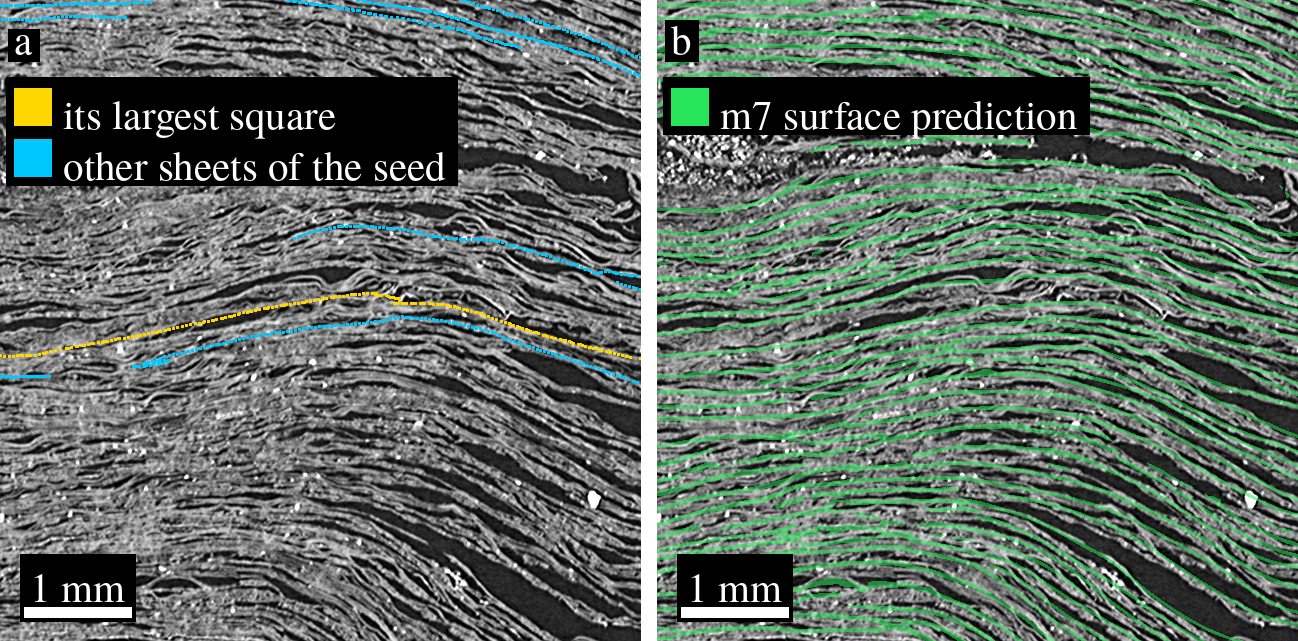
\includegraphics[width=\columnwidth]{figures/c-f10-papyrus}
\caption{\CaptionPapyrus}
\label{fig:papyrus}
\end{figure}

\subsection{Seeds}
\label{sec:seeds}

The prediction has a fault. On PHerc.~0826 only \PredInMask{} of the voxels it marks lie inside the scan's mask at the
coarsest level, against \PredInMaskRef{} on PHerc.~1447: it marks surface where the organisers masked the scan away,
often as solid blocks rather than sheets. We reported the blocks on PHerc.~1447 in villa issue 1875
(\UpVillaBlocksState{} when read on \UpReadAt{}). The seed rule avoids them. A seed is a voxel marked as surface whose
six face neighbours are marked, which lies on grey scan data, and whose prediction chunk is at most half marked. After
the first wave we added two tests, labelled as such in the declaration:\footnote{\texttt{src/prereg/chain-0826.md}.}
the seed must lie within the height range of the organisers' published umbilicus, and in a
chunk marked at most three tenths. The umbilicus enters the pipeline there and nowhere else; our own estimator of it is
studied in~\cite{workumbilicus} and is not run here. Each seed that passes is grown for a short fixed time, the ladder,
and a seed still growing at that cap is grown in full.

The first three waves draw uniformly from the prediction. The fourth, declared before the draw, draws around the
\NearSources{} seeds that had given a square of \SourceThreshold{}~mm or more, \NearPerSource{} draws around each and
\NearDraws{} in all, each between \NearShellMin{} and \NearShellMax{} voxels from its source point. Table~\ref{tab:waves}
counts every step. The fourth wave kept a larger share of its seeds through the ladder, \WaveFourYield{} of rule
passers against \WaveThreeYield{} in the third. Its seeds did not deliver larger squares: their median best square is
\WaveFourSquareMedian{}~mm against \WaveThreeSquareMedian{}~mm. It found far more squares per seed drawn than the
random waves (Figure~\ref{fig:yield}), but not more per machine hour (Section~\ref{sec:arms}). A fifth wave, declared
the same way, drew \NearFivePerSource{} draws around each of the \NearFiveSources{} seeds that had given
\NearFiveThreshold{}~mm or more, \NearFiveDraws{} in all, each at most \NearFiveShellMax{} voxels from its source.
One survivor of the fourth wave is neither delivered, crashed nor waiting (\AllNotDeliveredOther{} in all): its growth
ended and its downstream had not. The \WaveFiveWaiting{} survivors of the fifth wave had not been queued by the freeze, so
they count as waiting. We recomputed the best square of each delivered seed from its squares file, and it
agrees with the chain's own column on \SquareCheckAll{} seeds.

\begin{table*}[t]
\centering
\caption{The waves of PHerc.~0826 as run, at \ChainGenCap{} generations, frozen at the chain's relaunch
of \ChainFreezeTime{}. A crashed growth ended
with return code 139; a waiting seed survived the ladder and had not been grown to the end. The
square is the largest square fully covered on one delivered sheet, best over the seed's sheets. A
wave whose ladder has not grown all its rule passers says ``ladder unfinished''; the row over all waves
counts survivors per passer over the \WavesLadderFinished{} waves whose ladder is finished.}
\label{tab:waves}
\footnotesize
\setlength{\tabcolsep}{4pt}
\begin{tabular}{lrrrrrrrrrr}
\toprule
wave & draws & rule & ladder & survivors & delivered & crashed & waiting & median & largest & seeds \\
 & & passers & survivors & per passer & & & & square (mm) & square (mm) & at \SourceThreshold{}~mm \\
\midrule
1 & \WaveOneDraws & \WaveOnePassers & \WaveOneSurvivors & \WaveOneYield & \WaveOneDelivered & \WaveOneCrashed & \WaveOneWaiting & \WaveOneSquareMedian & \WaveOneSquareMax & \WaveOneSeedsTen \\
2 & \WaveTwoDraws & \WaveTwoPassers & \WaveTwoSurvivors & \WaveTwoYield & \WaveTwoDelivered & \WaveTwoCrashed & \WaveTwoWaiting & \WaveTwoSquareMedian & \WaveTwoSquareMax & \WaveTwoSeedsTen \\
3 & \WaveThreeDraws & \WaveThreePassers & \WaveThreeSurvivors & \WaveThreeYield & \WaveThreeDelivered & \WaveThreeCrashed & \WaveThreeWaiting & \WaveThreeSquareMedian & \WaveThreeSquareMax & \WaveThreeSeedsTen \\
4 & \WaveFourDraws & \WaveFourPassers & \WaveFourSurvivors & \WaveFourYield & \WaveFourDelivered & \WaveFourCrashed & \WaveFourWaiting & \WaveFourSquareMedian & \WaveFourSquareMax & \WaveFourSeedsTen \\
5 & \WaveFiveDraws & \WaveFivePassers & \WaveFiveSurvivors & \WaveFiveYield & \WaveFiveDelivered & \WaveFiveCrashed & \WaveFiveWaiting & \WaveFiveSquareMedian & \WaveFiveSquareMax & \WaveFiveSeedsTen \\
\midrule
all & \AllDraws & \AllPassers & \AllSurvivors & \AllYield & \AllDelivered & \AllCrashed & \AllWaiting & \AllSquareMedian & \AllSquareMax & \AllSeedsTen \\
\bottomrule
\end{tabular}
\end{table*}

\begin{figure}[t]
\centering
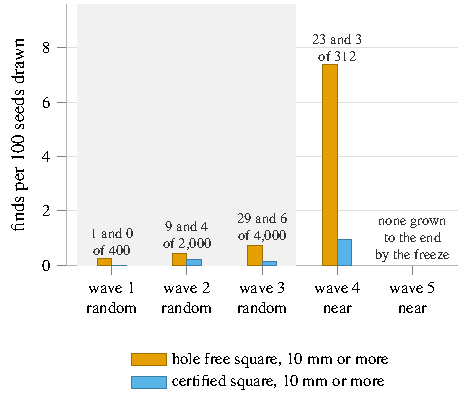
\includegraphics[scale=1]{figures/c-f19-yield-waves}
\caption{What each wave of the chain as run found, in the order the waves ran. It counts seeds with a square of
\SourceThreshold{}~mm or more on a delivered sheet, hole free (orange) or certified (sky blue), per
hundred seeds drawn, with the counts behind each pair above it. The shaded waves drew uniformly; the
fourth and fifth drew near earlier finds, and none of the fifth wave's seeds had been grown to the
end by the chain's freeze. The finds are those of the search yield comparison of
Section~\ref{sec:arms}. Drawn by \texttt{src/tools/c-f19-yield-waves.py} from
\texttt{src/evidence/figures/c-f19-yield-waves.csv}.}
\label{fig:yield}
\end{figure}

\subsection{The growth}
\label{sec:growth}

Stevens' usage text calls mode \texttt{g} ``generation, write patches and relationships''.\footnote{Line
\LineUsageG{} of his source at \SrCommit{}; the mode begins at line \LineG{} and calls the generator at line
\LineGGenerate{}.} From the seed it grows thousands of small patches of surface, each fitted to the prediction, and
records how neighbouring patches align. It is where the pipeline spends its time. The program takes the seed point and
the prediction as constants fixed when it is compiled,\footnote{\texttt{SEED\_X}, \texttt{SEED\_Y} and \texttt{SEED\_Z}
at lines \LineSeedX{}, \LineSeedY{} and \LineSeedZ{} of \texttt{pipeline9/parameters.h} at \SrCommit{}, with the seed's
axes after them; the prediction, \texttt{SURFACE\_ZARR}, at line \LineSurfaceZarr{}, which \texttt{simpaper10} opens at
line \LineSurfaceOpen{}.} so every seed needs its own build. We rebuild only the one object that reads them and link it
with the other \ObjEqualAcross{} objects. A build then costs \ObjPartialCpu{}~s of CPU against \ObjFullCpu{}~s for a
full rebuild, and its binary is byte identical to the full rebuild's (\ObjIdentical{}; measured on a PHerc.~1447 build
tree of the same source). On PHerc.~0826 the one object build equals a full build on \ObjCheckEqual{} of
\ObjCheckVariants{} build variants.
\ifRuntimeParamsDone
We then changed the program to read the seed from its environment when it runs, so that one binary serves every seed.
The change passes the same identity bar as every build: the build \RuntimeBuild{} against \RuntimeAgainst{}, identity
\RuntimeHolds{} on \RuntimeSeeds{}.
\else
Reading these values when the program runs, so that one binary serves every seed, is the next step we will offer to
Stevens; it is not part of this article.
\fi

To make the growth faster we rebuilt the same source with a flat hash for the patch lookup, AVX-512 kernels, link time
optimisation, profile guided optimisation and the native target, a build we call MLP. None of this may change a byte of
what is grown. Each build was admitted only if the new and the unchanged build grow the same three PHerc.~0826 seeds into
byte identical growth trees, sheets and stage files (Table~\ref{tab:identity}). The bar holds for MLP (\IdMlpHolds{})
and for the earlier flat hash and AVX-512 build (\IdHvHolds{}); for the latter one seed crashed on both builds and was
replaced (\IdHvReplaced{}). The chain's runner refuses a build without this bar.\footnote{The build gate of
\texttt{src/prereg/chain-0826.md}.}

The chain that delivered this article's sheets ran more than this build. Its program also carries \CorrOutput{}
corrections of defects in Stevens' source that change what is grown, and \CorrInert{} that were measured to change
nothing here. The arms of Section~\ref{sec:arms} leave them out, so that each arm changes one thing.\footnote{The nine
patches, with the source files each touches, under \path{src/inputs/chain-0826-corrections/}, listed by
\texttt{src/tools/corrections\_list.py} in \path{derived/corrections.csv}; arm X of
\path{src/prereg/stevens-changes-0826-91.md}.} The \CorrOutput{} that change output are a rounding made symmetric about
zero in the bad patch finder, a floor in place of a truncating cast in the sheet grid, positions taken relative to the
patch origin where the volume is indexed, and significant digits kept at the boundaries between stages. The other two
sort the chunk listing before it is indexed and write the right angle test of the matcher with the and that was meant.
The \CorrInert{} inert ones fix the absolute value of a boolean, make the renderer round instead of truncate, and choose
the transform that represents a pair by its translation. On the \CorrSeeds{} seeds of the arms, the chain's delivered
trees differ from arm~C's in growth patches on \CorrSeedsDiffer{} of them. Their medians are \CorrPatchesX{} growth patches
against \CorrPatchesC{}, a formula area of \CorrFormulaX{} against \CorrFormulaC{}~cm$^2$ and a best square of
\CorrSquareX{} against \CorrSquareC{}~mm. So what this article says of Stevens' pipeline as published, and of outputs
equal to it, holds for arms A, B and C only. Every sheet the checks judge in Sections~\ref{sec:checks} and~\ref{sec:out} comes from the chain with the
corrections.

\begin{table}[t]
\centering
\caption{Identity bars on PHerc.~0826: each build against the unchanged build, by file.}
\label{tab:identity}
\footnotesize
\begin{tabular}{llll}
\toprule
seed & growth tree & sheets & stage files \\
\midrule
\multicolumn{4}{l}{\emph{MLP against unchanged}} \\
109 & \IdMlpOneOhNineGrowth & \IdMlpOneOhNineSheets & \IdMlpOneOhNineStages \\
300 & \IdMlpThreeHundredGrowth & \IdMlpThreeHundredSheets & \IdMlpThreeHundredStages \\
237 & \IdMlpTwoThirtySevenGrowth & \IdMlpTwoThirtySevenSheets & \IdMlpTwoThirtySevenStages \\
\multicolumn{4}{l}{\emph{flat hash and AVX-512 against unchanged}} \\
109 & \IdHvOneOhNineGrowth & \IdHvOneOhNineSheets & \IdHvOneOhNineStages \\
300 & \IdHvThreeHundredGrowth & \IdHvThreeHundredSheets & \IdHvThreeHundredStages \\
237 & \IdHvTwoThirtySevenGrowth & \IdHvTwoThirtySevenSheets & \IdHvTwoThirtySevenStages \\
\bottomrule
\end{tabular}
\end{table}

We timed the builds on a quiet machine, one growth at a time with the arms alternating, on seed 237
(Table~\ref{tab:clock}). A run counts only if it returned zero, its tree was identical, and no other growth ran beside
it. The rule, declared before the runs, is that the new arm's median must fall below the old arm's minimum. For MLP
against the flat hash and AVX-512 build the verdict is \ClkMlpRuleCpu{} on CPU time and \ClkMlpRuleWall{} on wall time,
with factors of \FacMlpCpu{} and \FacMlpWall{}.\footnote{CPU medians of \FacMlpCpuOld{} and \FacMlpCpuNew{}~s, the
first two rows of Table~\ref{tab:clock}.} For the LZ4HC copy against the zstd copy, both under MLP, the verdict is
\ClkLRuleCpu{} and \ClkLRuleWall{}. What the whole acceleration does on PHerc.~0826 is arm C against arm B of
Section~\ref{sec:arms}.

\begin{table}[t]
\centering
\caption{Quiet clocks of one growth, PHerc.~0826 seed 237, in seconds; hash, AVX-512 is the flat hash
and AVX-512 build. Runs: counted runs; others: the most cores other processes held during a counted
run of that arm.}
\label{tab:clock}
\footnotesize
\setlength{\tabcolsep}{3pt}
\begin{tabular}{llrrrrrr}
\toprule
 & & & & \multicolumn{2}{c}{CPU} & \multicolumn{2}{c}{wall} \\
build & copy & runs & others & median & min & median & min \\
\midrule
hash, AVX-512 & zstd & \ClkHvCounted & \ClkHvOthersMax & \ClkHvCpuMed & \ClkHvCpuMin & \ClkHvWallMed & \ClkHvWallMin \\
MLP & zstd & \ClkMlpCounted & \ClkMlpOthersMax & \ClkMlpCpuMed & \ClkMlpCpuMin & \ClkMlpWallMed & \ClkMlpWallMin \\
\midrule
MLP & zstd & \ClkZCounted & \ClkZOthersMax & \ClkZCpuMed & \ClkZCpuMin & \ClkZWallMed & \ClkZWallMin \\
MLP & LZ4HC & \ClkLCounted & \ClkLOthersMax & \ClkLCpuMed & \ClkLCpuMin & \ClkLWallMed & \ClkLWallMin \\
\bottomrule
\end{tabular}
\end{table}

We also found a defect in the growth. When the generator places the seed cells of a new patch it does not reset their
velocities, so a patch depends on the patch grown before it. The fix, a reset we call SetSeed, changes what is grown. On
PHerc.~0826 it shortened the growth of each of the three seeds we tried: by Stevens' formula (Section~\ref{sec:formula}),
seed 6365 went from \DeliveredSixThreeSixFive{} to \SetSeedAFormula{}~cm$^2$, seed 2019 from \DeliveredTwoOhOneNine{} to
\SetSeedBFormula{}~cm$^2$ and seed 5630 from \DeliveredFiveSixThreeOh{} to \SetSeedCFormula{}~cm$^2$.
Figure~\ref{fig:setseed} shows one of them before and after, and arm D against arm C gives the effect over the paired
seeds. A second defect, mode \texttt{g} reusing an output folder without checking it, is scrollreading issue 2
(\UpSrTwoState{}). The villa surface tracer is an alternative to this growth. Our correction of its seed is villa pull request 1915
(\UpVillaSeedZeroState{}), and villa issue 1914 (\UpVillaRayIssueState{}) describes the cost that a second correction
changed.

\begin{figure}[t]
\centering
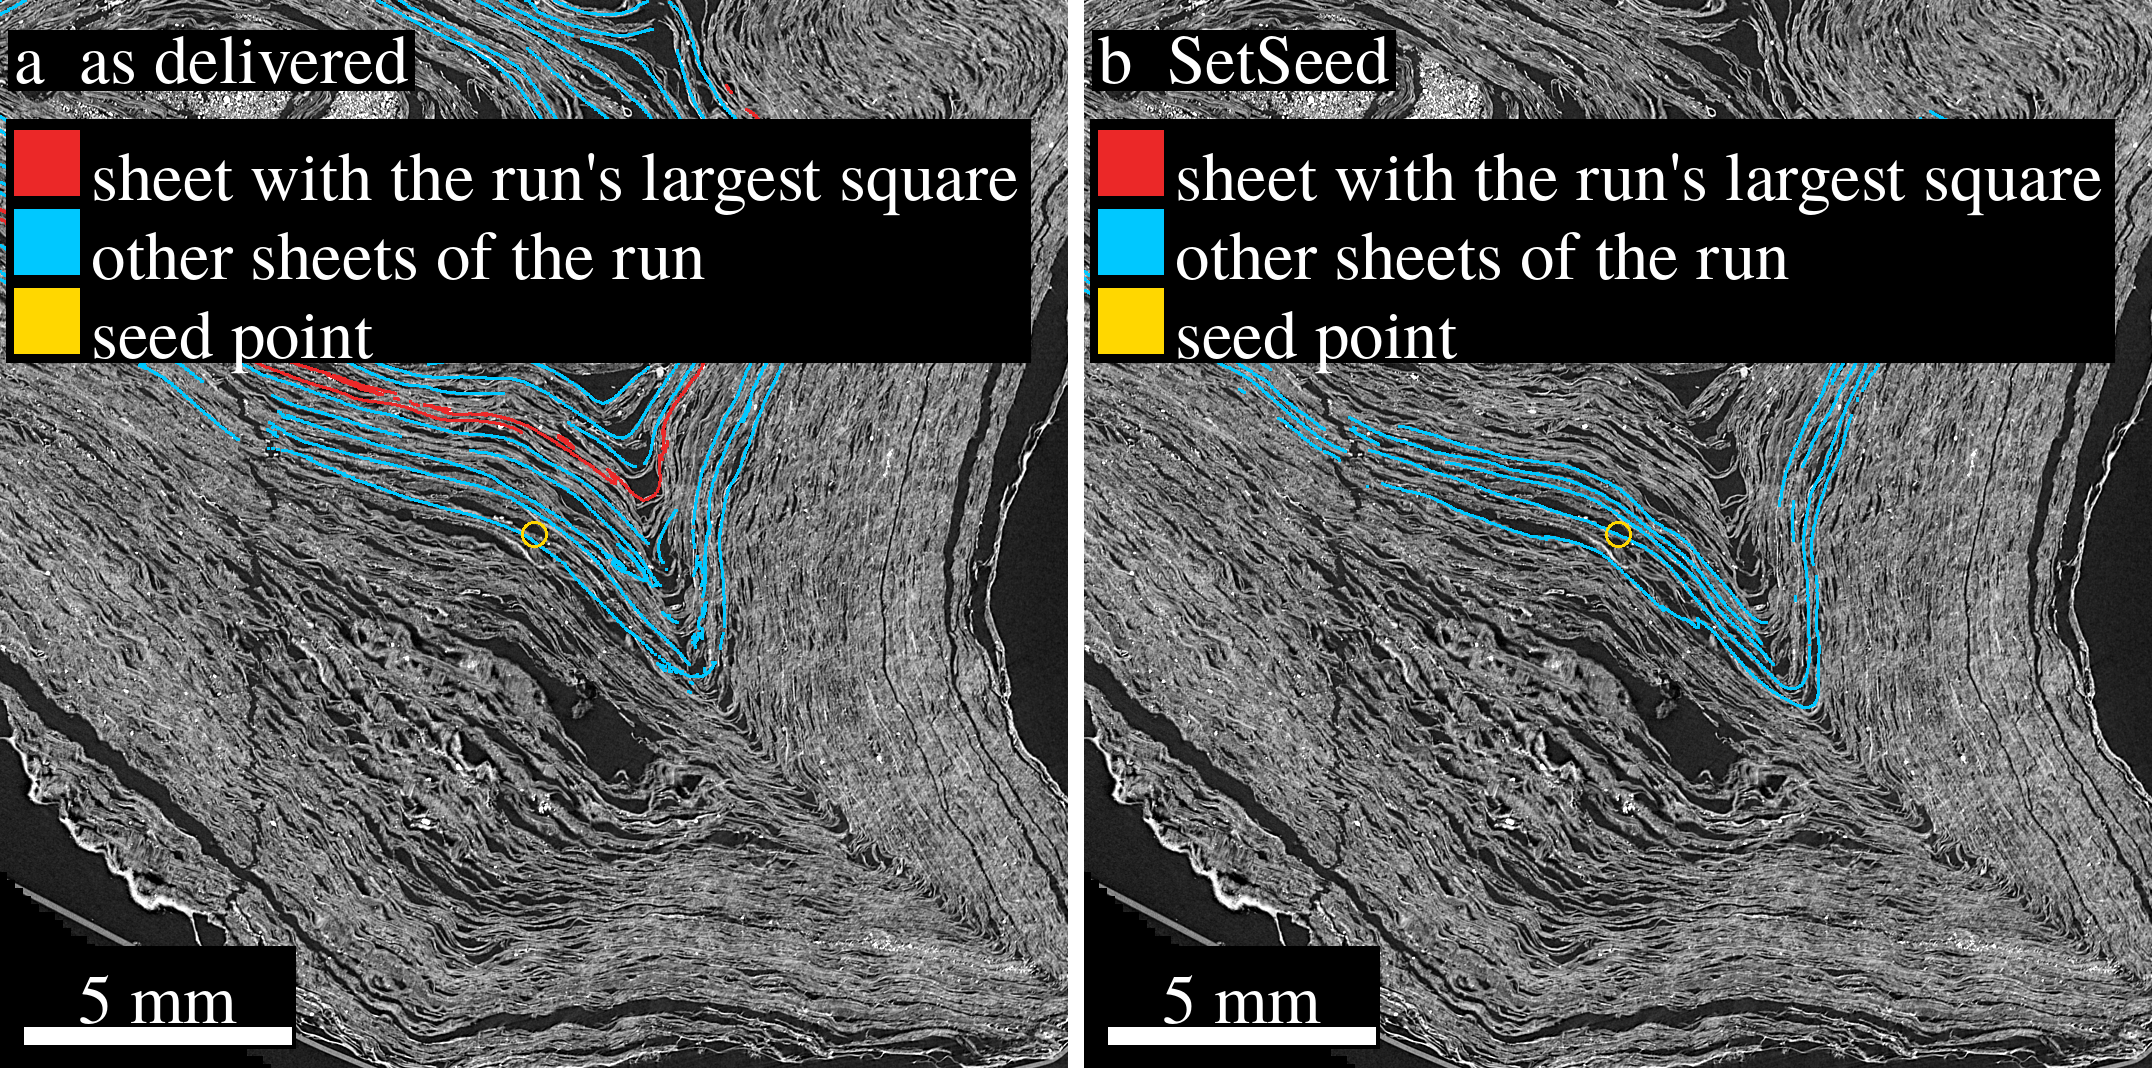
\includegraphics[width=\columnwidth]{figures/c-f13-setseed}
\caption{\CaptionSetSeed}
\label{fig:setseed}
\end{figure}

\subsection{The downstream stages}

The bad patch finder, mode \texttt{c}, removes the patches whose alignments contradict each other. It looks for chains
of alignments that should close on themselves and do not.\footnote{Mode \texttt{c} begins at line \LineC{} of Stevens'
source; its rounds are lines \LineCRoundTwo{} to \LineCRoundFive{}.} On large trees it could run for hours or be
abandoned. Two changes inside one function make it finish while writing the same files, and a guard turns an abort into
a result. They are measured on Stevens' own scrolls in~\cite{workS} and proposed as scrollreading pull requests 3
(\UpSrThreeState{}) and 4 (\UpSrFourState{}); on PHerc.~0826 their effect is arm B against arm A. The four stages that
join the kept patches into connected components, settle them with a spring simulation and write each component as one
flattened sheet run as Stevens published them.\footnote{Lines of Stevens' source at \SrCommit{}. Mode \texttt{l} is at
\LineL{} and its centres at \LineLCentre{}. Mode \texttt{vm} is at \LineVm{}, its ordering at \LineVmOrders{} and its
bridges at \LineVmBridges{}. Mode \texttt{hm} is at \LineHm{}, its springs at \LineHmSprings{} and \LineHmRun{}. Mode
\texttt{fm} is at \LineFm{}, its sheets at \LineFmScore{}.} ScrollFiesta is a different mesher of the same prediction.
Our pull requests 17 (\UpSfSeventeenState{}), 18 (\UpSfEighteenState{}) and 21 (\UpSfTwentyOneState{}) and issues 19
(\UpSfNineteenState{}) and 20 (\UpSfTwentyState{}) of its repository concern its stage costs and the faults its winding
gate misses.

\section{The checks and the certified square}
\label{sec:checks}

This section says what the checks are, what they certify on PHerc.~0826, where they fail, and what they do not
establish about ink.

A delivered sheet can cross from one lamina to the next, and three tests look for that. The a2 test flags the points
where a sheet runs steeper than \AtwoTstar{} degrees against the surface prediction; its cluster rule cuts every
cluster of more than \AtwoS{} flagged points out of the sheet before the square is measured again. Over all delivered
sheets, \AllAtwoShare{} of the measurable points are flagged. The rule sees steep crossings and not a gradual drift, so
the crossing map between sheets and the self-conflict test see more. Two sheets conflict when they run parallel at about
one pitch apart over at least \LaminaConflictArea{} square voxels; the pitch is \LaminaPitch{} voxels, within
\LaminaConflictPitches{} pitch. A sheet that conflicts with itself folds onto the next winding, and this is the one
lamina test. A hole free square with no cell that crosses a compared sheet, conflicts with its own surface or lies in
a cluster the a2 rule cuts is certified (Section~\ref{sec:intro} names the sheets compared), and
Figure~\ref{fig:certified} shows the largest on our own sheets. Figure~\ref{fig:atwo} shows the sheet where the cluster
rule costs most.

\begin{figure*}[t]
\centering
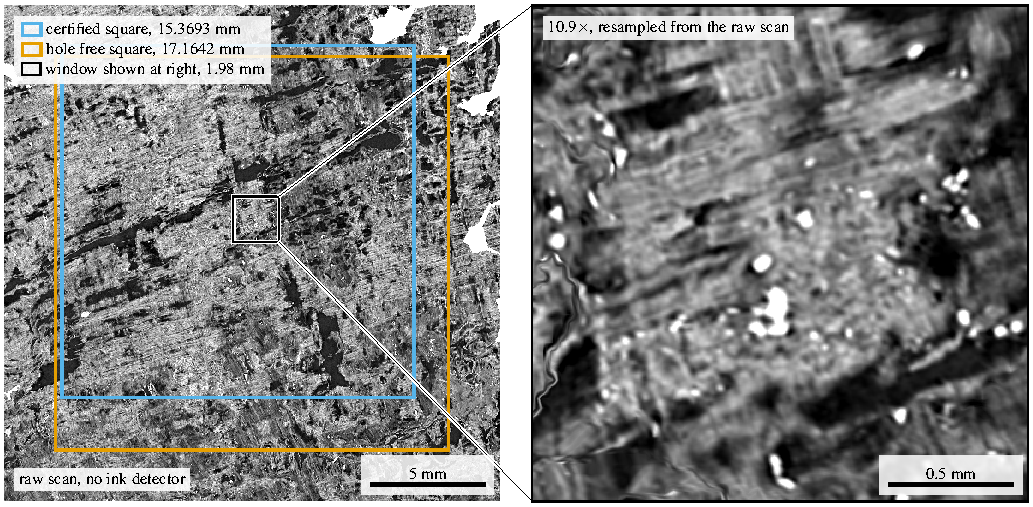
\includegraphics[width=0.85\textwidth]{figures/c-f16-certified-square}
\caption{\CaptionCertifiedSquare}
\label{fig:certified}
\end{figure*}

\begin{figure}[t]
\centering
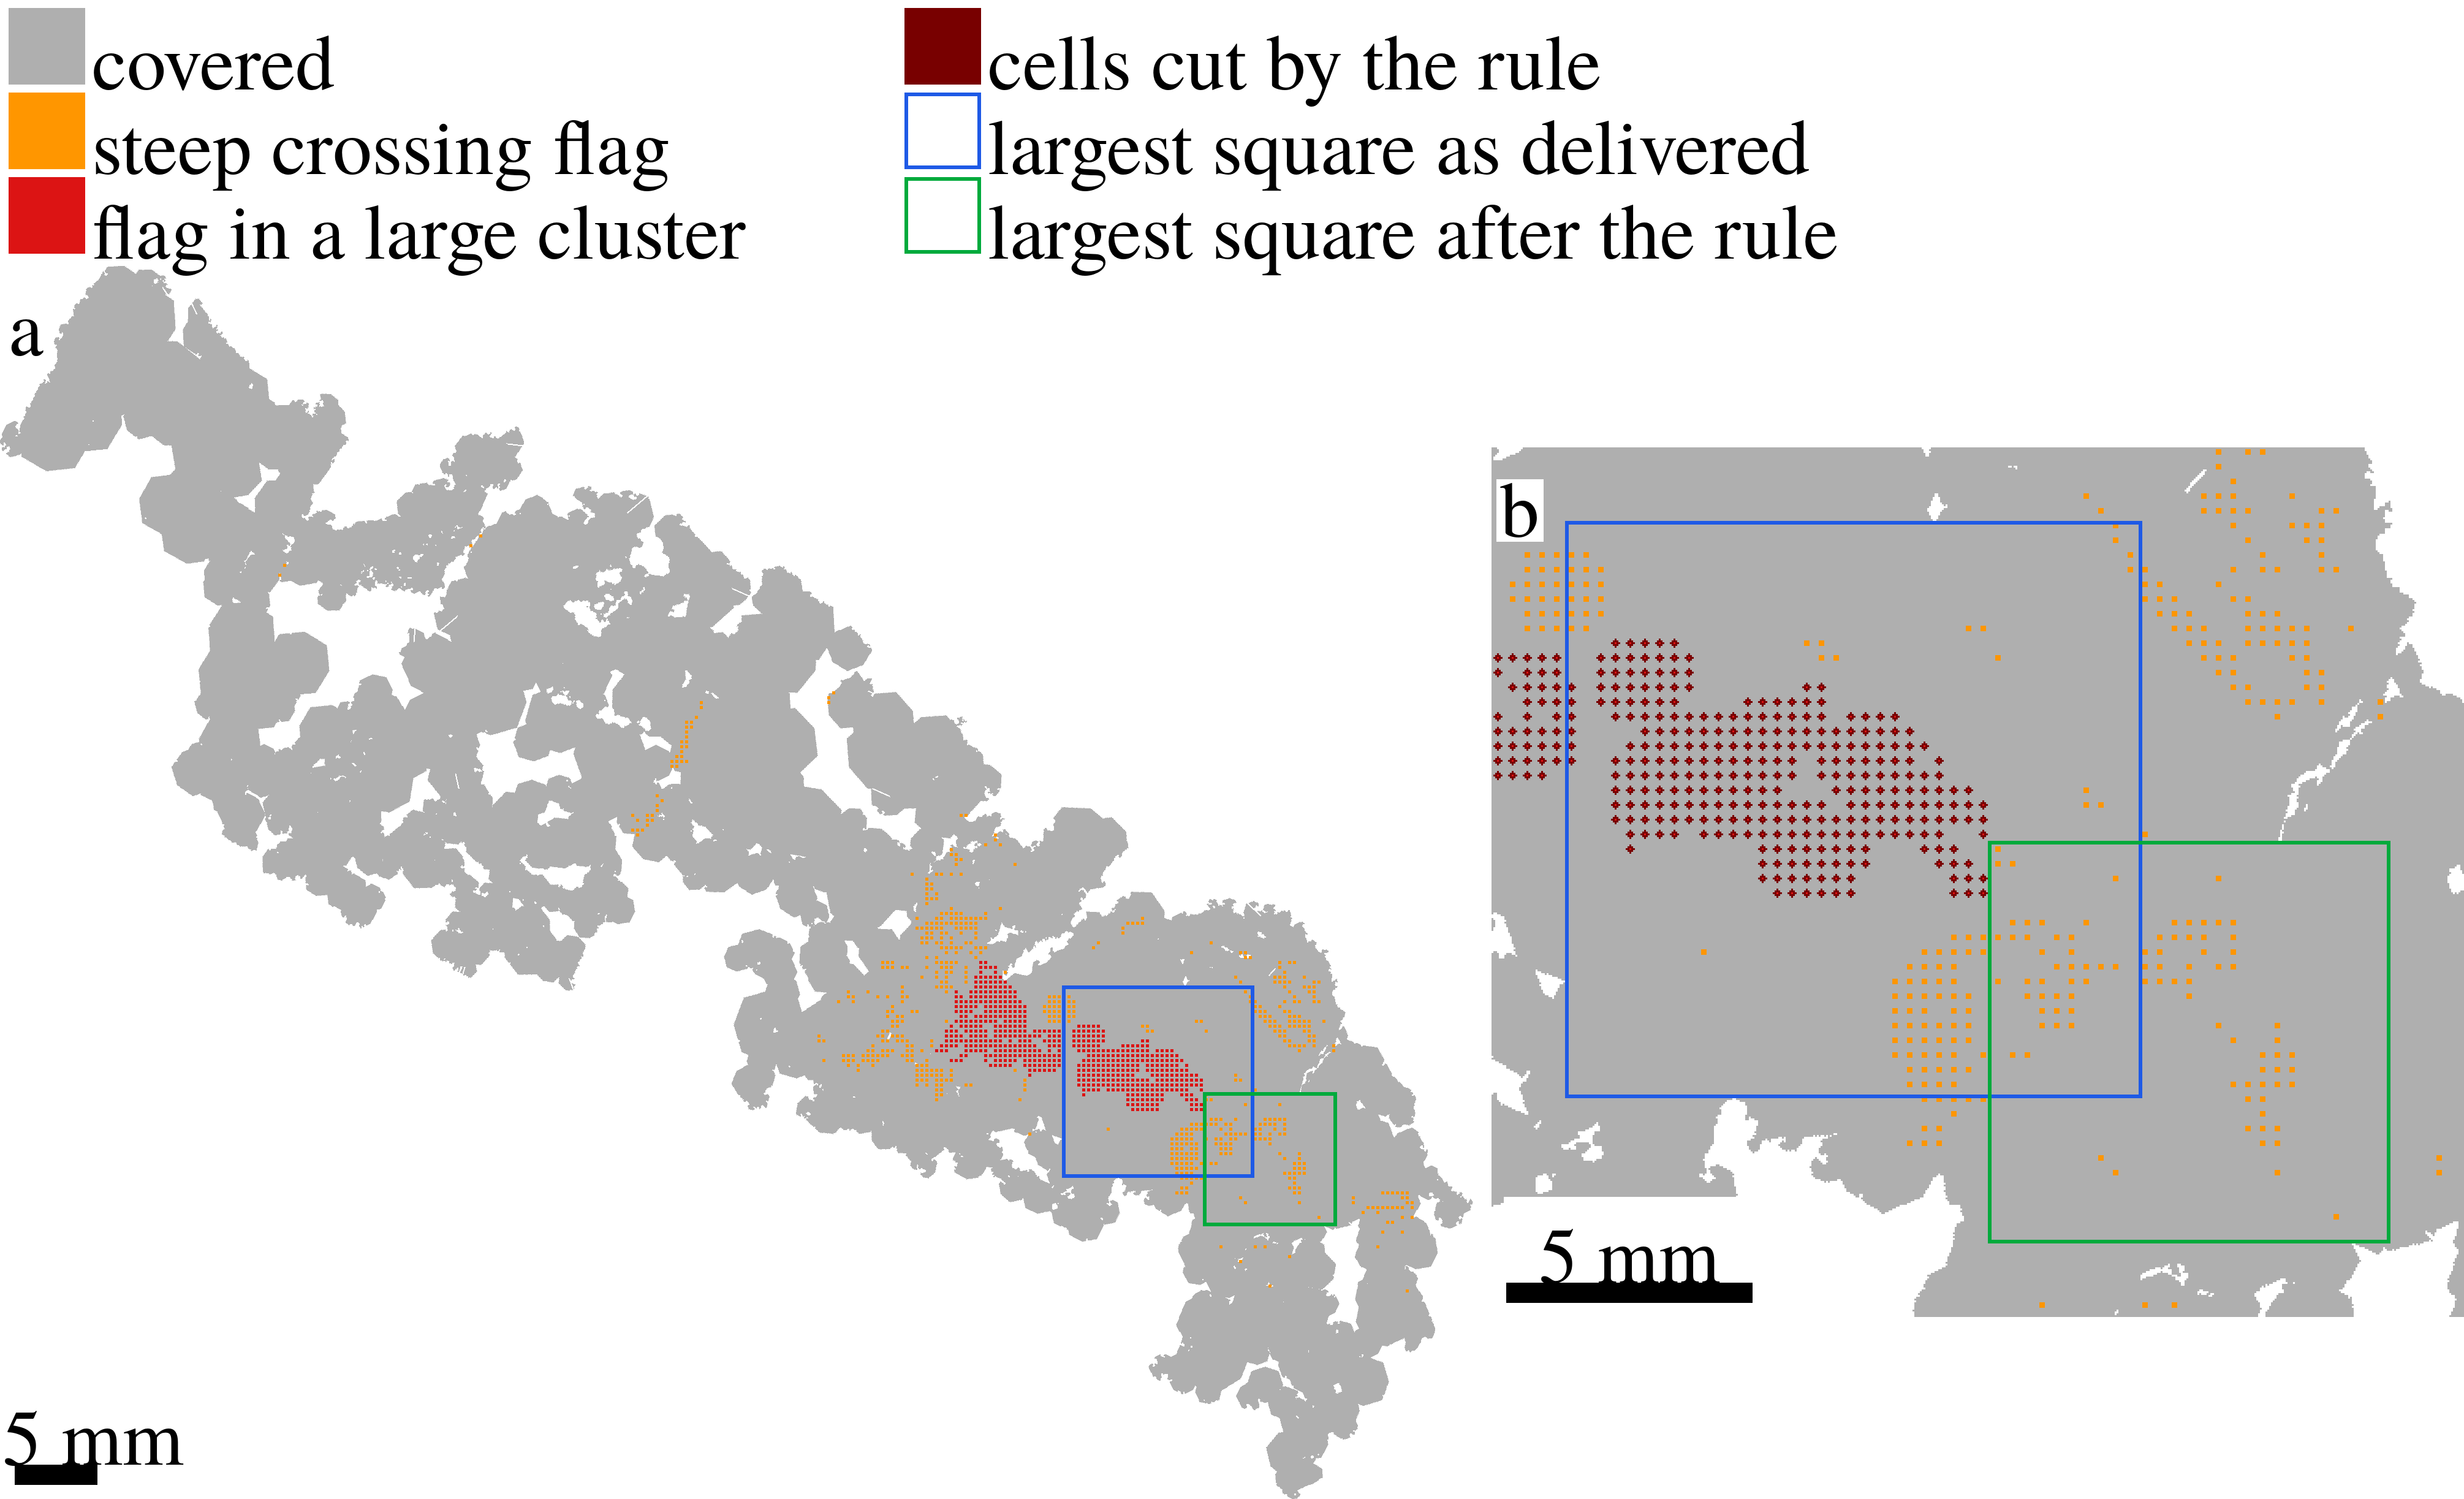
\includegraphics[width=\columnwidth]{figures/c-f12-a2-flags}
\caption{\CaptionAtwoFlags}
\label{fig:atwo}
\end{figure}

A conflict test says where two sheets do not lie on one lamina; it does not say that a piece lies on the surface of
papyrus. The raw scan shows the fibres of a papyrus surface as bands along two directions, and we score that on every
certified piece of \FibrePopulationMin{}~cm$^2$ or more, \FibrePiecesRanked{} pieces. They are pieces of the chain's
sheets and of the longer regrowths of Section~\ref{sec:out}, pooled. In each of \FibreWindows{} random
windows of \FibreWindowCells{} by \FibreWindowCells{} grid cells inside the piece we take the share of the raw scan's
spectral power at periods of \FibrePeriodMin{} to \FibrePeriodMax{}~mm along the two grid axes. The fibre score is the
median of those shares. On \FibrePiecesFewerWindows{} pieces fewer windows fit inside, and on
\FibrePiecesNotMeasurable{} none fits, so these have no score and do not pass. White noise scores \FibreWhiteNoise{}.
The piece whose fibres we see by eye, \FibreReferenceSheet{}, scores \FibreReference{}, and the bar for papyrus surface
is \FibreBarFactor{} of that, \FibreBar{}. Of the \FibrePiecesRanked{} pieces, \FibrePiecesPassing{} pass it. The
largest certified square on a sheet that passes is \FibreBestSquare{}~mm (\FibreBestSquareSheet{}, fibre score
\FibreBestSquareScore{}).

\subsection{The certified square}

The checks judge a surface, not the program that made it, and the headline square of this article comes from a surface
we did not grow. Our search gave the start, the centre of the certified square of seed \RcOneSeedId{}, and the
organisers' tracer grew a surface from it for \RcOneGenerations{} generations. Our checks ran on a crop of \RcCrop{} by
\RcCrop{}~mm around the start, against our own delivered sheets and against the tracer's other surfaces. Where two
traced surfaces cross, the crossing counts against the one that agrees less with our delivered sheets there. The largest
square they certify is \RcOneSquare{}~mm on a side (Figure~\ref{fig:r2c}). Inside it no cell crosses one of the \UnionSheets{} sheets,
no crossing with another traced surface counts against it, none is in conflict with the surface itself at one pitch,
none lies in a cluster the a2 rule cuts and none is a hole.

Before the adjudication the largest square on this surface was \RcOneSquareBefore{}~mm, and a cross section inside it, at
a crossing decided against this surface, shows the part the adjudication removes running along a void rather than
along papyrus. Measured on that earlier square, the fibre score is \RcOneFibre{}, over the bar of \FibreBar{}. A
share \RcOneOnOurs{} of its nodes lie within \StraightNear{} voxels of our own delivered sheet \RcOneOurSheet{}, so the
tracer and our chain found the same layer there. Its straightened sections give medians of \RcOneSecIMedian{} and
\RcOneSecJMedian{} voxels, with shares \RcOneSecIShare{} and \RcOneSecJShare{}. The same route from the centre of the
certified square of seed \RcTwoSeedId{} gives \RcTwoSquare{}~mm, fibre score \RcTwoFibre{}. A first measure of the same
start on a crop of half that side had given \RcOldSquare{}~mm. On the whole crop that square holds self-conflicts whose
other end lies outside the smaller crop, and it carries no other flag. So the number is \RcOneSquare{}~mm, and it is the
checks, run on the larger crop with crossings between traced surfaces adjudicated, that set it.

A larger square passes the same checks. Route R2d grew the same tracer from the square centres of more of our
sheets, and on the one from sheet 0 of seed 2715 the square certified with crossings adjudicated is
\RdSquare{}~mm.\footnote{Row \texttt{R2dnative} of seed 2715 in
\path{src/inputs/render-routes-0826/square-three-definitions.csv}, column \texttt{c\_certified\_adjudicated\_mm}, and
\path{candidate-2715.csv} beside it; route R2d and the adjudication rule are additions to
\path{src/prereg/render-routes-0826.md}.} Axial cuts
through it show that its dark corner runs through air: a run of at least \CutsVoidRun{} nodes off papyrus lies on each
of the \CutsRdCrack{} cuts at the crack, and on none of the \CutsRdStreaks{} cuts at dark streaks or the
\CutsRdControls{} controls.\footnote{Study \texttt{cuts-2715}, declared in \path{src/prereg/cuts-2715.md} with the
heights withheld; \path{verdict.csv}; the values in \path{derived/cuts-summary.csv}.} Whether the surface changes layer
at the crack, and whether it stays on one layer across the streaks, the cuts leave undecided. The checks certified it
all the same, so it is not the headline square, and it is a limit of the checks.

\subsection{Where the checks reject the pipeline's best}

What the checks caught on this scroll is the reason to run them. The \FibreTopFailCount{} largest certified pieces,
the sheets that look best by their size (\FibreTopFailPieceMin{} to \FibreTopFailPieceMax{}~cm$^2$), score
\FibreTopFailScoreMin{} to \FibreTopFailScoreMax{} on the fibre test, under its bar of \FibreBar{}. The largest
passing piece is \FibreBestPiece{}~cm$^2$ (\FibreBestPieceSheet{}, fibre score \FibreBestPieceScore{}), which is the
reference sheet itself; the largest passing piece on any other sheet is \FibreBestOtherPiece{}~cm$^2$
(\FibreBestOtherPieceSheet{}, fibre score \FibreBestOtherPieceScore{}).
\ifSquareChecksCrossing
The largest hole free square the pipeline grew, \RegrowBest{}~mm on a side, folds onto the next winding inside itself,
and the largest square on that sheet that avoids the fold is \CheckLaminaAvoid{}~mm (Section~\ref{sec:out}).
\else
The largest hole free square the pipeline grew, \RegrowBest{}~mm on a side, is not certified one lamina
(Section~\ref{sec:out}).
\fi

The checks also run together as one tool that returns, with no person choosing, the places worth reading. A window is a
square of at least \WinSide{}~mm on a side, \WinArea{}~cm$^2$, on one delivered sheet, measured in the sheet's own grid.
It is clean when at least \WinCoveredBar{} of its cells are covered and at most \WinFlaggedBar{} are flagged by any of
the checks, and when its fibre score is at least \WinFibreBar{}, taken over whole tiles of \WinTileCells{} by
\WinTileCells{} cells. The rule was declared before the search ran.\footnote{Study \texttt{best-windows-0826}, its
declaration \path{src/prereg/best-windows-0826.md} and its tool \texttt{bw.py}, shipped under \path{src/tools/studies/}; \path{windows.csv} and
\path{attempts.csv}.} The search went through the \WinSheets{} certified pieces that pass the fibre test, which lie on
\WinSheetsDistinct{} sheets of \WinSeedsSearched{} seeds. On \WinCandidateSheets{} sheets some window meets the
coverage and flag bars. Of those, \WinCleanSheets{} hold a clean window, from \WinCleanSeeds{} different seeds. On the
other \WinCandidateNotClean{}, too few whole tiles fit between the holes to give a fibre score; no window failed because
a score fell under the bar. The best one, on sheet \WinBestSheet{} of seed \WinBestSeedId{}, has a flagged share of
\WinBestFlagged{}, covers \WinBestCovered{} of its cells and scores \WinBestFibre{} over \WinBestTiles{} tiles. The
search's own self-tests, \WinSelfTests{} of them on synthetic cases, all pass. Figure~\ref{fig:windows} shows the best
three windows, on seeds \WinBestThreeSeeds{}. In the sheet's own grid the axis nearer the scan's height lies
\WinAngleMin{} to \WinAngleMax{} degrees from it, so the windows are also shown resampled with rows at constant height by
the window study's own tool \texttt{align.py}.

\begin{figure*}[t]
\centering
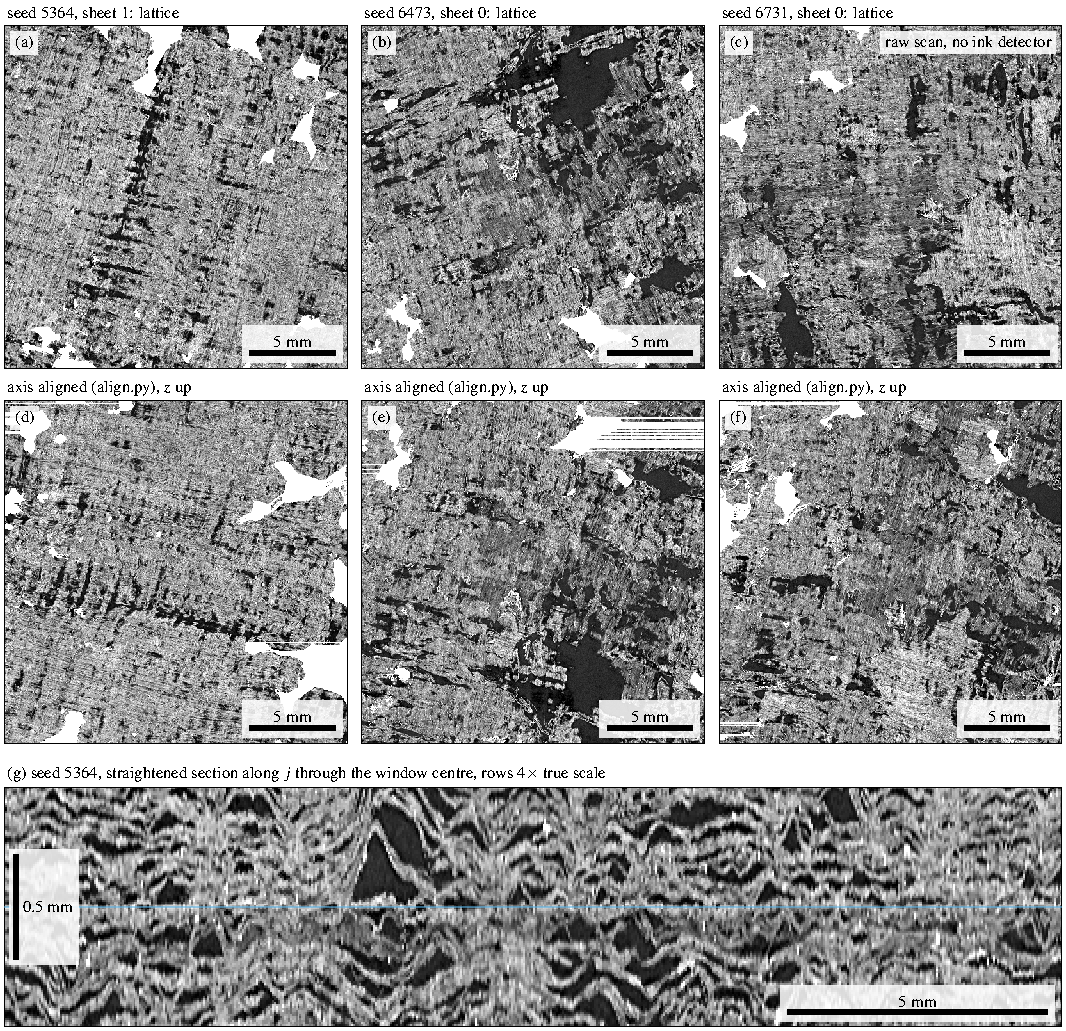
\includegraphics[width=0.88\textwidth]{figures/c-f20-best-windows}
\caption{\CaptionBestWindows}
\label{fig:windows}
\end{figure*}

The raw scan can also be asked, along the sheet itself, whether a sheet stays on one layer. For the best three windows we
straightened the scan along each grown point's normal on the two lines of the window through its centre, and took the
offset of the brightest voxel within \StraightWindow{} voxels of the sheet in each column. A peak placed at random would
lie a median of \StraightRandomMedian{} voxels from the sheet, and within \StraightNear{} voxels in a share
\StraightRandomShare{} of the columns; that is arithmetic, not a measured null. On the two lines of the best window the
medians are \StraightOneIMedian{} and \StraightOneJMedian{} voxels and the shares \StraightOneIShare{} and
\StraightOneJShare{}, so there the brightest layer sits near the traced sheet more often than a random peak would. The
other two windows, and the certified square of Figure~\ref{fig:certified}, give medians of \StraightOtherMedMin{} to
\StraightOtherMedMax{} voxels and do not separate from a random peak on both lines. The window of \StraightWindow{}
voxels holds about two neighbouring laminae at a pitch of \LaminaPitch{} voxels, so a brighter neighbour can win a
column while the sheet stays on its own layer. A section that passes is not proven to lie on one layer.

\subsection{Ink: a positive control, and none on PHerc.~0826}

The checks say which surface to keep; they do not say that a surface they keep can be read. We asked that of the whole
loop on a scroll whose ink is labelled, PHerc.~0139, in a clean labelled region of \PcRegion{}~cm$^2$. The same binary
and settings as on PHerc.~0826 grew our sheets from seeds inside that region. The same render path and the released ink
model~\cite{inkmodel} read two of our sheets and, the same way, the organisers' own segment of that region. They were
read in every in plane orientation, both depth directions and both released checkpoints, \texttt{seed42} and \texttt{seed43}, \PcReadsA{} reads of each
sheet. Our base render of \RefSegments{} of their labelled segments matches their surface volumes with a normalised
cross correlation of \RefNcc{}, with no turn and no offset. The score is the balanced accuracy on the labelled pixels
that both surfaces reach within \PcMatch{} voxels. On the first sheet the best read reaches \PcOursABa{}, against
\PcTheirsABa{} for the organisers' segment on the same \PcCommonA{} pixels; on the second, \PcOursBBa{} against
\PcTheirsBBa{} on \PcCommonB{} pixels. Each sheet was also read as a null: copies of the same surface moved along its
normal into the dark gap on either side, \PcNullReadsA{} null reads per sheet. The best null reaches \PcNullA{} and
\PcNullB{}, under the sheets' own best reads, so our sheets carry the labelled ink to the ink model.

Our reads of PHerc.~0826 could not use labels, which that scroll does not have; they used a label free statistic that
compares the ink model's output on the sheet with its output on the same nulls. On the known ink of PHerc.~0139, run on
squares of \PcLabelFreeSquare{}~mm of our two sheets, of which the labelled region of \PcRegion{}~cm$^2$ covers only a part,
that statistic says no on all \PcLabelFreeRows{} of its rows, and
yes on \PcLabelFreeYes{}. A statistic that does not see ink where the labels show it cannot say anything of a scroll
without labels, so our reads of PHerc.~0826 with this model are \PcInkReading{}. The labelled
region was the organisers' validation region while the model was trained, and its labels reach our scan through a
fitted affine map. Both limit what this control can say.\footnote{Study \texttt{positive-control-0139}: its declaration \path{src/prereg/positive-control-0139.md},
\path{verdict.csv} (appended, never rewritten), \path{control.csv}, \path{null-best.csv} and \path{labelfree-w016.csv},
with the tools \texttt{score.py}, \texttt{verdict.py}, \texttt{null\_best.py} and \texttt{labelfree\_table.py}.}

We also read the two squares with a second model, v8-in, which Nader released with its code and weights under the MIT
licence~\cite{v8in}. Its depth order matters, and the order that suits our renders is not stated, so we measured it on the
organisers' surface of the w016 region of PHerc.~0139. On \VeinOrderPixels{} clean held out label points the balanced
accuracy is \VeinOrderBa{} in one order and \VeinOrderBaOther{} in the other. The side of each surface against the
scroll's axis carries the better order to PHerc.~0826, as a rule of geometry and not as a measurement there.
Figure~\ref{fig:veinw} shows the model on that labelled region, on the organisers' surface and on our sheet.\footnote{Studies
\texttt{selftrain-v8in-0826} and \texttt{ink-v8in-0826}, declared in \path{src/prereg/}; \texttt{selftrain-v8in-0826} (\path{order-0139.csv}, tool \texttt{w016.py}) and \texttt{ink-v8in-0826}
(\path{hf-files.csv}, \path{describe-v2.csv}, \path{ratio-calibration.csv}, tools \texttt{hf\_files.py},
\texttt{upright\_full.py} and \texttt{ratio\_cal.py}); the values in \path{derived/v8in-summary.csv}.}

We read the whole squares of seeds \RcOneSeedId{} and \RcTwoSeedId{}, as they stood before the adjudication, in both
orders. Each read has two null copies beside it: the same surface moved along its normal into the gaps on either side,
read the same way. The copies are not independent nulls: each shares \VeinNullSharedMin{} to \VeinNullSharedMax{} of
the \VeinNullLayers{} layers the model reads with the sheet. In the order measured on w016, counted over the pixels of
the square's render covered by the sheet and both copies, the share of pixels at probability \VeinThreshold{} or more is
\VeinSixSheet{} on the sheet of seed \RcOneSeedId{}, against \VeinSixPlus{} and \VeinSixMinus{} on its copies. For seed
\RcTwoSeedId{} it is \VeinFiveSheet{}, against \VeinFivePlus{} and \VeinFiveMinus{}. In the other order, counted over the nodes of the square's aligned grid, the sheet of seed
\RcOneSeedId{} gives \VeinSixSheetOther{}, against \VeinSixPlusOther{} and \VeinSixMinusOther{}. That of seed
\RcTwoSeedId{} gives \VeinFiveSheetOther{}, against \VeinFivePlusOther{} and \VeinFiveMinusOther{}. Layers moved
\VeinFaceOffset{} voxels towards either face of the sheet of seed \RcOneSeedId{} give \VeinFacePlus{} and
\VeinFaceMinus{} in the order measured on w016, over the same grid. On the known ink of w016 the share on the sheet over the larger of its
two copies runs from \VeinRatioMin{} to \VeinRatioMax{} across the organisers' surface and our two sheets. On
PHerc.~0826, over the render pixels of the shares above, it is \VeinRatioSix{} and \VeinRatioFive{}, inside that spread, and since on known ink the sheet can score
below its copies, the ratio decides nothing here. We, the authors, looked at these maps by eye and see no letter forms in any of them.
Figure~\ref{fig:veinsquare} shows those of the square grown from seed \RcOneSeedId{}'s start, as it stood before the
adjudication, the square the shares above are counted on, in both orders. Table~\ref{tab:veinreads} lists every read
of PHerc.~0826 with this model, \VeinReadsCount{} so far, each in the pixel set it was counted on. We also read the whole
surface that the organisers' tracer grew on route R2d from sheet 0 of seed 2715, in the order measured on w016: a share
\VeinRdShare{} of its \VeinRdPixels{} render pixels is at probability \VeinThreshold{} or more, and since no null
copies of that surface were read, the share has nothing to be set against. In the other order the same surface gives a share
\VeinRdShareOther{} over the same pixels, again with no null copies read; looking at that map by eye we see no letter
forms, and the share claims nothing. Figure~\ref{fig:veinmore} shows the maps of these two reads and of the square of seed
\RcTwoSeedId{} in both orders. The reads of PHerc.~0826 remain
\PcInkReading{}.

\begin{figure*}[t]
\centering
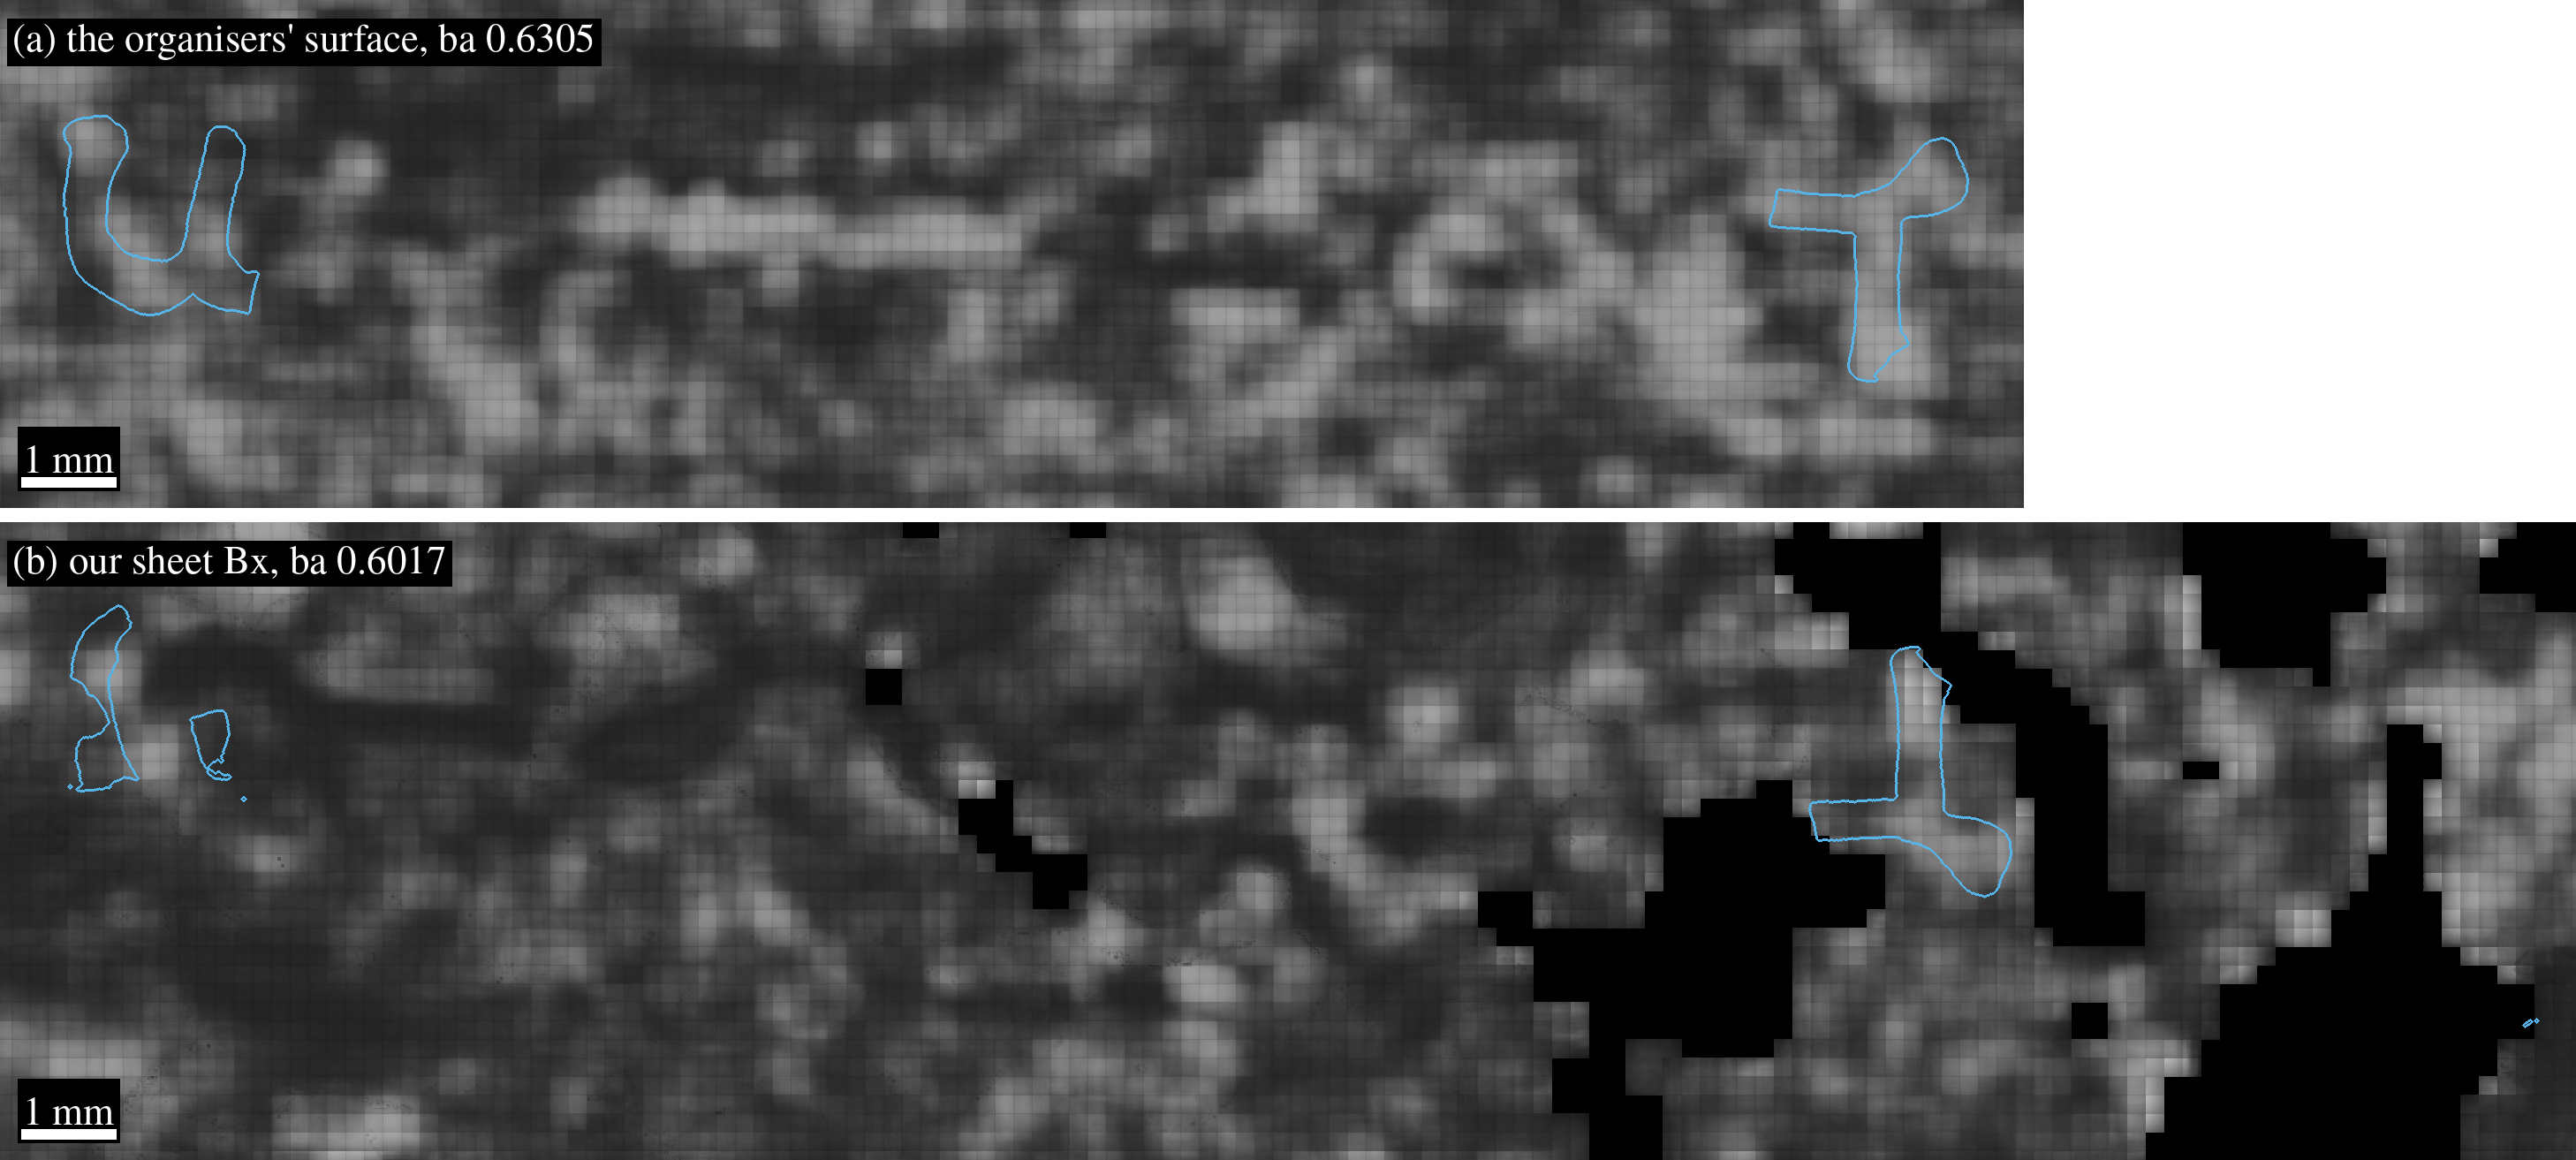
\includegraphics[width=\textwidth]{figures/c-f22-v8in-w016}
\caption{\CaptionVeinW}
\label{fig:veinw}
\end{figure*}

\begin{figure*}[t]
\centering
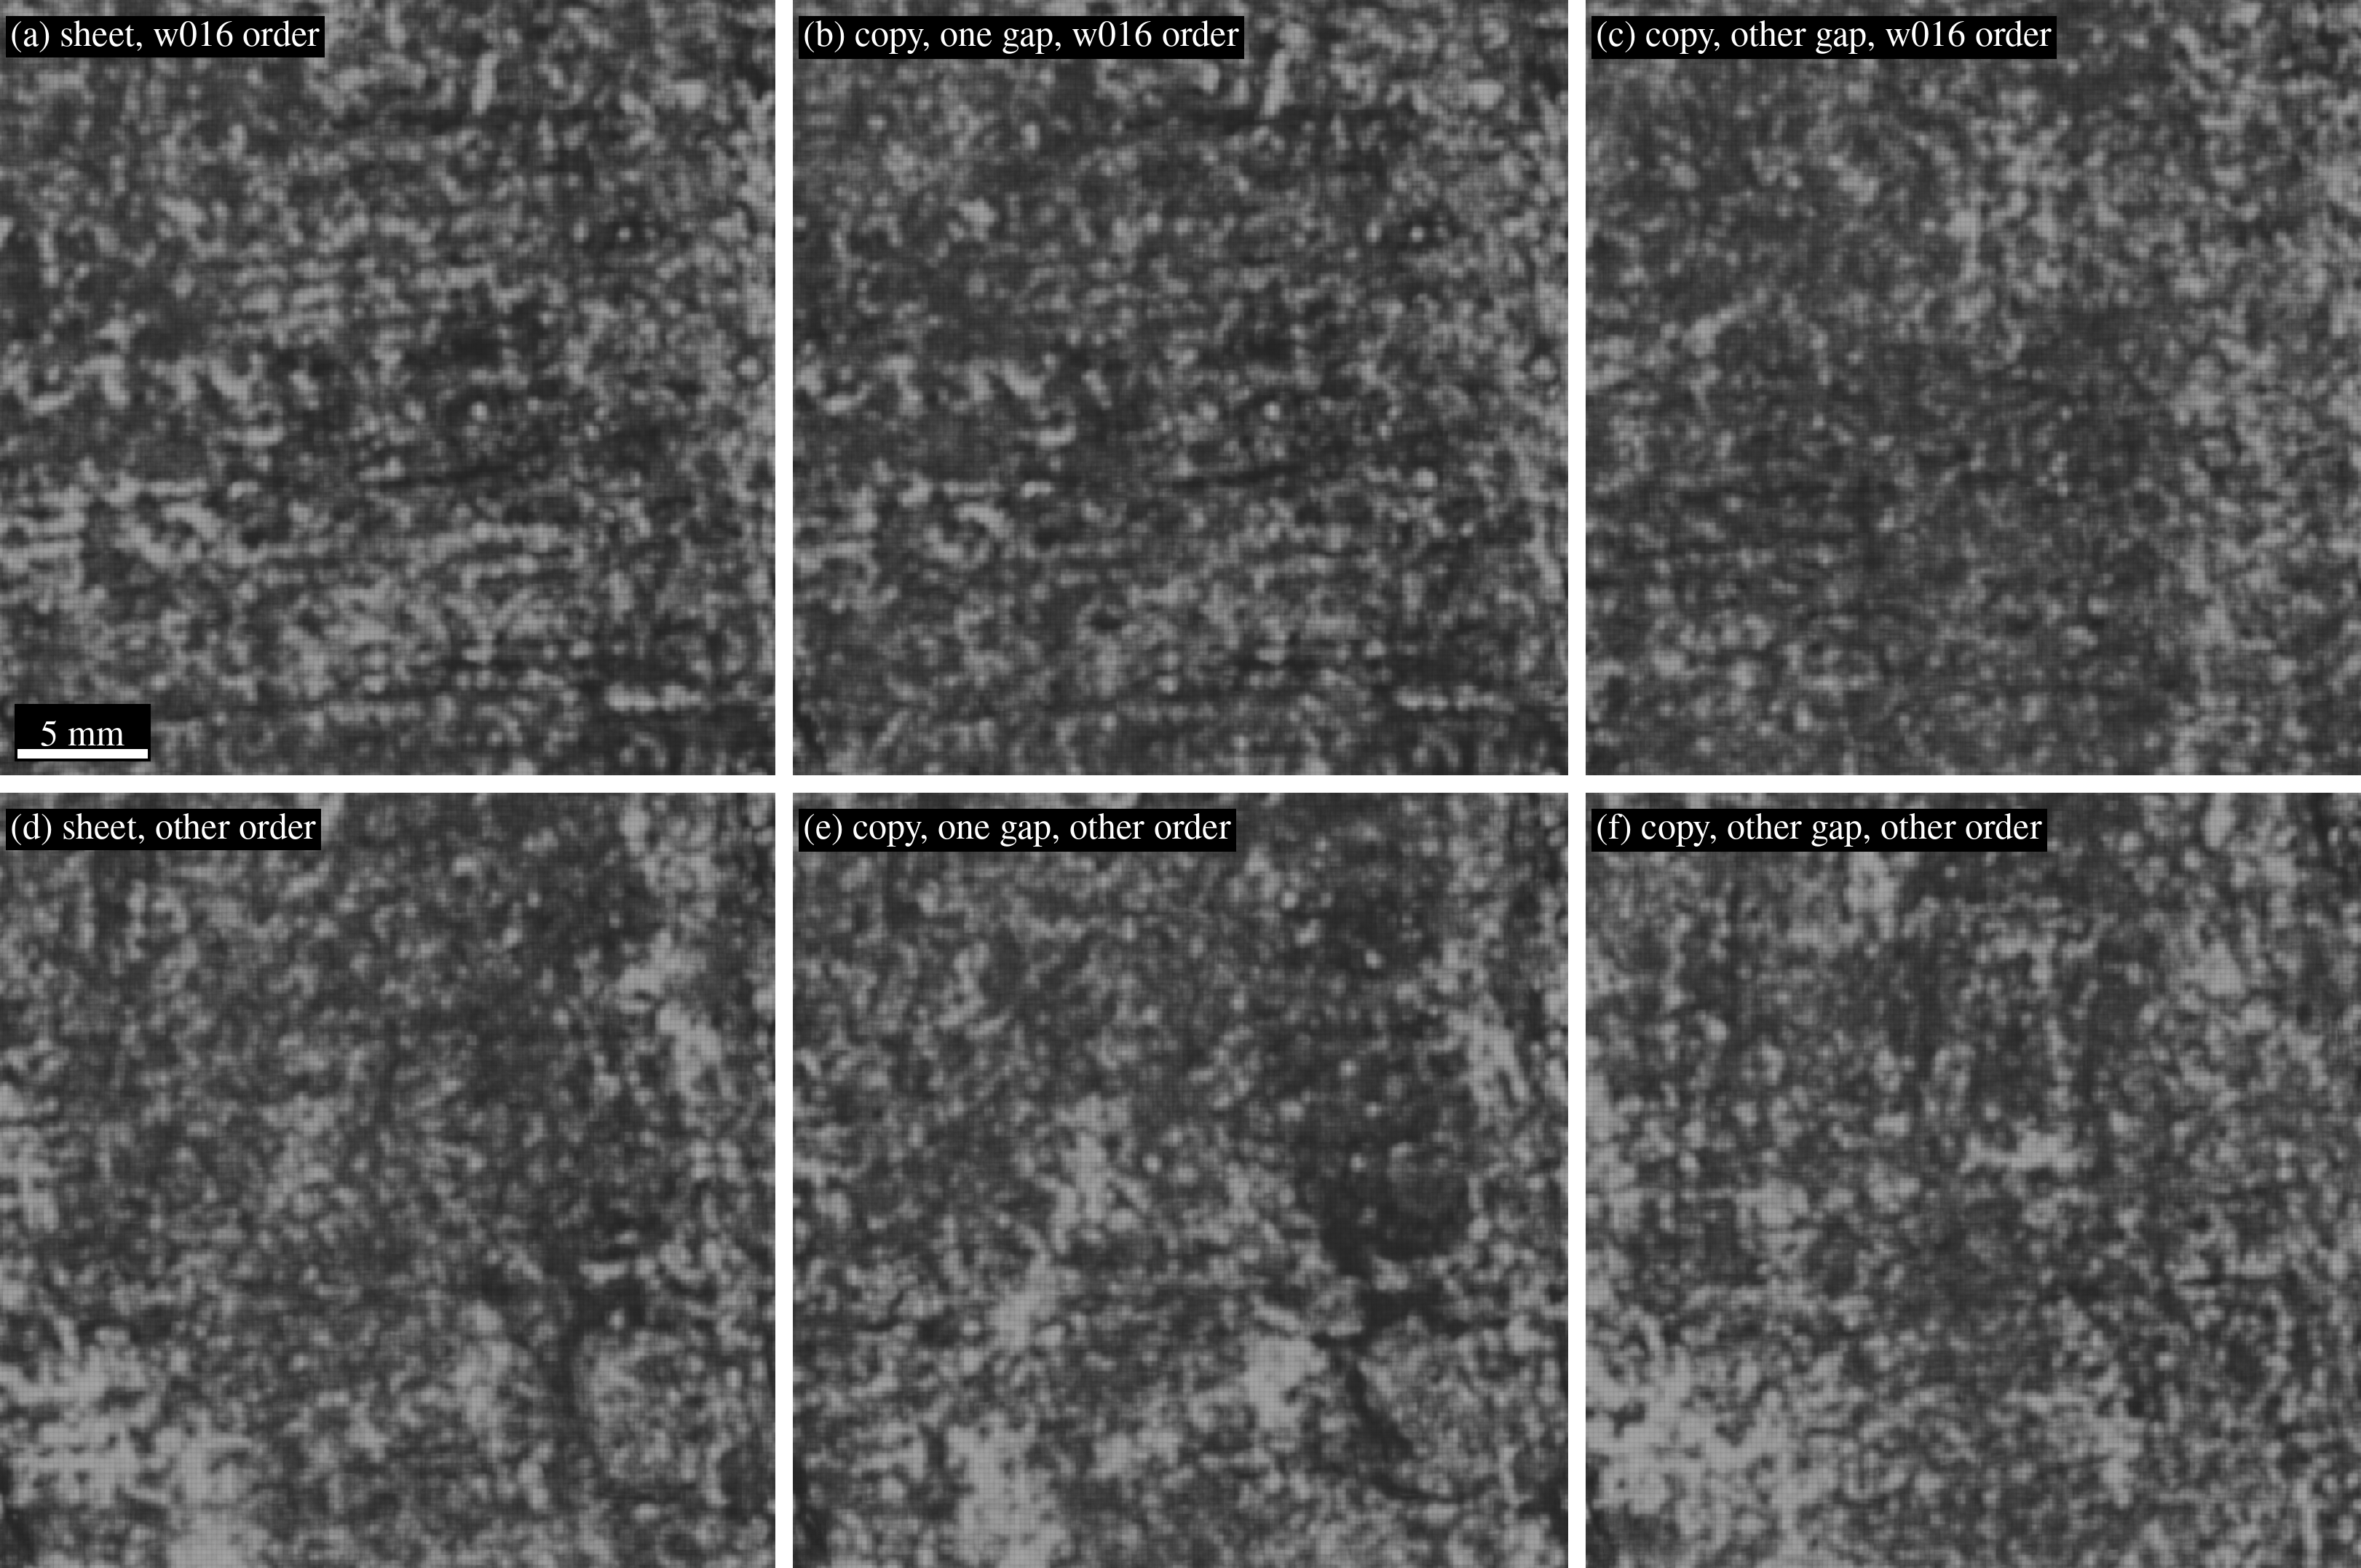
\includegraphics[width=\textwidth]{figures/c-f23-v8in-0826}
\caption{\CaptionVeinSquare}
\label{fig:veinsquare}
\end{figure*}

\begin{figure*}[t]
\centering
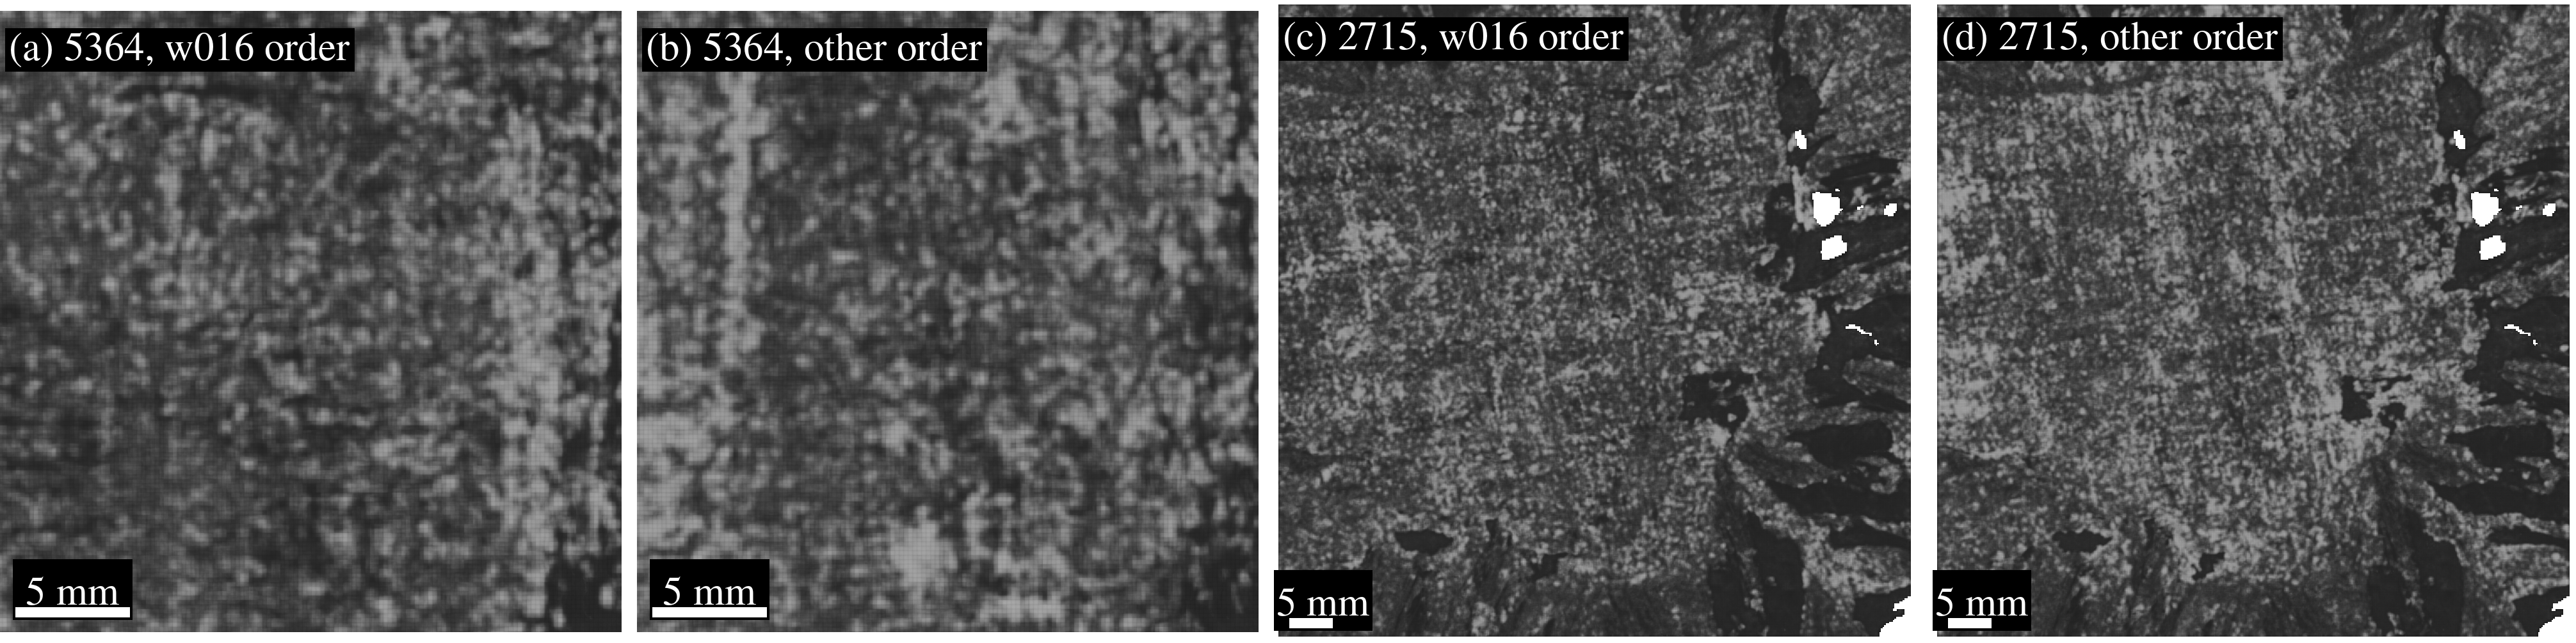
\includegraphics[width=\textwidth]{figures/c-f24-v8in-more}
\caption{\CaptionVeinMore}
\label{fig:veinmore}
\end{figure*}

\begin{table*}[t]
\centering
\caption{v8-in reads on PHerc.~0826, one row per read, uncalibrated and descriptive. The share is of the pixels scored
at probability \VeinThreshold{} or more, on the sheet and on each of its two null copies, and the last column is the
sheet's share over the larger copy's. The squares are counted over the nodes of their aligned grid, so their shares in
the order measured on w016 differ from those the text gives over the square's render pixels; the whole surface is
counted over the render pixels its read covers, and its null copies were not read. From
\texttt{derived/v8in-reads.csv}, written by \texttt{src/tools/v8in\_reads.py}.}
\label{tab:veinreads}
\footnotesize
\setlength{\tabcolsep}{4pt}
\begin{tabular}{lllrrrrr}
\toprule
surface & extent & depth order & pixels & sheet & null copy & other copy & sheet over \\
 & & & scored & share & share & share & larger copy \\
\midrule
\VeinReadsRows
\bottomrule
\end{tabular}
\end{table*}

\section{What the chain delivered}
\label{sec:out}

The \AllDelivered{} delivered seeds gave \AllSheets{} sheets, and Figure~\ref{fig:square} shows the best square of each
seed. The median is \AllSquareMedian{}~mm and the largest is \AllSquareMax{}~mm. Of these seeds, \AllSeedsTen{} reach
\SourceThreshold{}~mm; at 20~mm the count is \AllSeedsTwenty{} seeds and \AllSheetsTwenty{} sheets. Under the a2 cluster
rule the median best square is \AllClusterMedian{}~mm and the largest \AllClusterMax{}~mm, and \AllClusterSeedsTen{}
seeds keep a square of \SourceThreshold{}~mm or more. Figure~\ref{fig:where} shows where the best of them sit relative
to each other.

\begin{figure}[t]
\centering
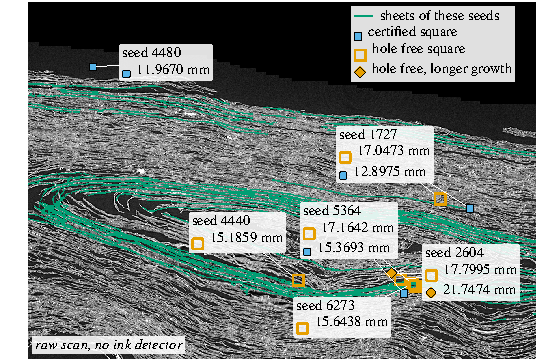
\includegraphics[width=\columnwidth]{figures/c-f17-where-squares}
\caption{\CaptionWhereSquares}
\label{fig:where}
\end{figure}


\begin{figure*}[t]
\centering
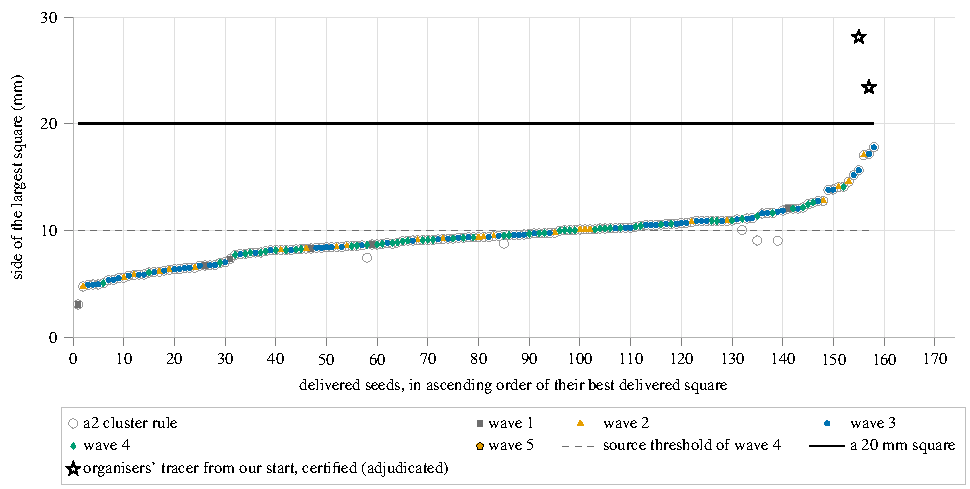
\includegraphics[width=\textwidth]{figures/c-f2-best-square}
\caption{The best square of each delivered PHerc.~0826 seed, as delivered (filled marks, one per
wave) and under the a2 cluster rule (grey rings), seeds in ascending order of the delivered square.
The dashed line is the source threshold of the fourth wave and the solid line the side of a
20~mm square. The open stars are the certified squares of the organisers' tracer grown from our chosen starts
(Section~\ref{sec:checks}), under the adjudicated definition, each above the seed whose certified square gave its start.
The other marks are the chain's own growths at \ChainGenCap{} generations; the regrowths of
\RegrowSeeds{} seeds at \RegrowGenCap{} are in the text, not in this figure. Plotted numbers: \texttt{src/evidence/figures/c-f2-best-square.csv}.}
\label{fig:square}
\end{figure*}

The best seeds had stopped at the growth cap of \ChainGenCap{} generations rather than by themselves, so we grew them
again for longer. Every seed whose best square was \NearFiveThreshold{}~mm or more had stopped at that cap:
\RegrowAtCap{} of \RegrowSeeds{}. We grew them again from the same seed for \RegrowGenCap{} generations, with the same
binary and settings, and ran the downstream stages with a patch limit of \RegrowPatchLimit{}, which keeps every
generation. None of these regrowths enters the chain's counts, medians or maxima above, but the fibre test of
Section~\ref{sec:checks} pools their pieces with the chain's. The step was declared
before any of them.\footnote{Study \texttt{square20-0826-95}, declared in \path{src/prereg/square20-0826-95.md}. The chain itself grows at \RegrowGenCap{} since its
relaunch of \ChainFreezeTime{}; the \ChainSeedsAfterFreeze{} seeds it started since are in neither set.} Up to the old
cap each regrowth repeats the first growth (\RegrowIdentity{} for the seed below), and all \RegrowEnded{} ended by
themselves before the new cap. Seed \RegrowBestSeed{} had given a best square of \RegrowBestBefore{}~mm. Its regrowth
reached generation \RegrowBestGeneration{}, and one of its sheets now holds a hole free square of \RegrowBest{}~mm on a
side (\RegrowBestCells{} cells on the grid of sheet \RegrowBestSheet{}). Under the a2 cluster rule it stays
\RegrowBestCluster{}~mm. The other seeds' best squares are between \RegrowOthersMin{} and \RegrowOthersMax{}~mm. We
also regrew the \RegrowNextSeeds{} next capped seeds the same way. Of all these regrowths, only \RegrowBestSeed{}'s best
square changed by more than \RegrowNextChange{}~mm.\footnote{Study square20-0826-95:
\path{square20-0826-95/cap-check-next10.csv}, rows with regrow yes, and each seed's squares file before (g
\ChainGenCap{}) and after (g \RegrowGenCap{}). Among the next \RegrowNextSeeds{} the largest change is
\RegrowNextChangeSeed{}'s, from \RegrowNextChangeBefore{} to \RegrowNextChangeAfter{}~mm, and among the other seeds of
the first group the largest is \RegrowOthersChange{}~mm (\RegrowOthersChangeSeed{}). Computed by
\texttt{src/tools/square95.py}.} The square is hole free, not certified one lamina.
\ifSquareChecksClean
The crossing map between sheets and the one lamina test found no crossing inside it at the cut off; that is what those
tests can see, not a certificate.
\else\ifSquareChecksCrossing
Both tests found a crossing inside it by the cut off. The one lamina test flags cells where the sheet folds onto the
next winding, and the largest square avoiding them is \CheckLaminaAvoid{}~mm. The crossing map against the other sheets
also flags cells inside it, and the largest square avoiding those is \CheckVtwoAvoid{}~mm.
\else
The crossing map between sheets and the one lamina test on this sheet were not complete at this article's cut off of
\CutoffTime{}, declared before it.
\fi\fi
The chain as run delivers no square of 20~mm.

Squares measure one place; area measures how much surface the pipeline found, counting overlaps between sheets once.
The area was measured on the \AreaSeeds{} seeds delivered when that study froze its set. A cell is clean when it is
covered, not flagged by a2 and not on a crossing line between two sheets. Clean cells of different sheets that fall on
the same place are counted once, and of three rules for ``the same place'' we quote the smallest result. Over
\UnionSheets{} sheets the clean area is \UnionOneStep{}~cm$^2$; the other two rules give \UnionHalfStep{} and
\UnionBinMax{}~cm$^2$, and summed without deduplication it would be \UnionCleanSummed{}~cm$^2$. This area is coverage,
not one lamina, and it is not filtered by the fibre test. The sheets of one seed wind through several laminae, so it
counts surface on many windings. Joined along their overlaps without a conflict, the largest group holds
\LaminaGroup{}~cm$^2$ of clean area over \LaminaGroupSheets{} sheets of \LaminaGroupSeeds{} seeds. The \LaminaWrapping{}
sheets that conflict with themselves are left out, and \LaminaRefusals{} merges are refused because they would put two
windings in one group. Its best member has a square of \LaminaGroupSquare{}~mm.

\subsection{Stevens' formula on the PHerc.~0826 runs}
\label{sec:formula}

Stevens reports his result as an area on another scroll: PHerc.~1667, ``around~\StevensQuoted{}~cm$^2$ of
coverage''~\cite{winners}. His repository has no area tool; the number is the sum, over the \StevensComponents{}
flattened components of one run, of each component's grid cells times its two cell steps, with overlaps counted and no
crossing cleaned. We reproduce it on his components as \StevensRepro{}~cm$^2$ and use the same formula only to describe
our own runs, not to compare them with his. Over the \FormulaRuns{} growth runs, one seed each, the best single run,
\FormulaBestRunSeed{}, gives \FormulaBestRun{}~cm$^2$, and the sum over all runs, which counts every overlap, is
\FormulaSumRuns{}~cm$^2$ (Figure~\ref{fig:formula}). Four delivered seeds pooled as one run and passed through the
downstream with no cap give \CollFourFormula{}~cm$^2$ over \CollFourSheets{} components, and \CollFourUnion{}~cm$^2$
deduplicated and cleaned. The seed with the best single run, put through the same route alone, gives
\CollControlFormula{}~cm$^2$, against \DeliveredSixThreeSixFive{}~cm$^2$ as delivered by the chain. The fibre test
scored \FibreCollFourPiecesRanked{} certified pieces from the \FibreCollFourSeeds{} pooled seeds,\footnote{Seeds from
\path{src/prereg/area-0826-90.md}, the declared collection; pieces from \path{certified-piece-0826/fibre-ranking.csv} (declared in \path{src/prereg/certified-piece-0826.md}),
every certified piece of \FibrePopulationMin{}~cm$^2$ or more; rows \texttt{fibre\_coll\_four\_*} of
\path{derived/fibre-summary.csv}.} so this pooled area is not shown to be papyrus surface.

%% PENDING-BEGIN road 1b
% Which paragraph prints is decided by src/tools/cutoff.py at the declared cut off, never here.
\ifRoadOneBRun
The route was repeated on a wider collection. The rule declared first took the \RoadOneBSeeds{}
delivered seeds nearest the best one. It chose them among the \RoadOneBQualified{} seeds with a
square of \SourceThreshold{}~mm or more. Before the launch the list was cut to the nearest
\RoadOneBSeedsUsed{}, for time and memory. The run pools those \RoadOneBSeedsUsed{} seeds and
\RoadOneBPatches{} patches. Its smallest best square is \RoadOneBUsedMinSquare{}~mm, and its farthest
seed lies \RoadOneBUsedMaxDistance{} voxels from the best one. Pooled as one run it gives
\RoadOneBFormula{}~cm$^2$ by the same formula and a largest square of \RoadOneBSquare{}~mm. The a2 test
flags \RoadOneBAtwo{} of its points, and \RoadOneBVtwo{} cells lie on crossing lines.
\else
The route was to be repeated on a wider collection. The rule declared first took the \RoadOneBSeeds{}
delivered seeds nearest the best one. It chose them among the \RoadOneBQualified{} seeds with a
square of \SourceThreshold{}~mm or more. Before the launch the list was cut to the nearest
\RoadOneBSeedsUsed{}, for time and memory, which made \RoadOneBPatches{} patches. That run did not
finish, because in the bad patch stage its memory grew without bound. On its third pass its memory went from
\RoadOneBPassThreeGB{}~GB to \RoadOneBStopGB{}~GB. That took \RoadOneBStopMinutes{} minutes, on
\RoadOneBStopPatches{} patches. It was stopped at the \RoadOneBBound{}~GB bound declared before the
run, as an earlier attempt had been at \RoadOneBFirstBound{}~GB. We report this as a limit of the bad
patch stage at this size, not a result, and the four seed collection above is the widest pooled run
reported here.
\fi
%% PENDING-END

\begin{figure*}[t]
\centering
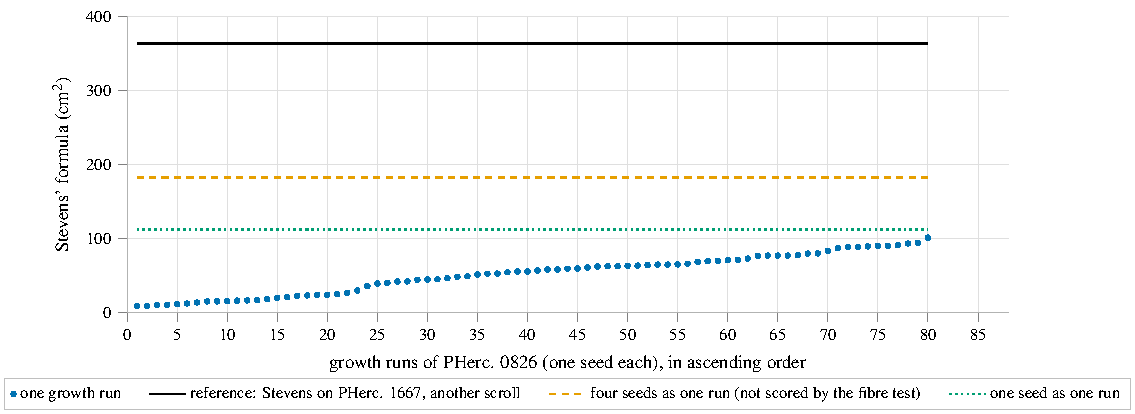
\includegraphics[width=\textwidth]{figures/c-f3-stevens-formula}
\caption{Stevens' formula on each PHerc.~0826 growth run, in ascending order, and on the four seed run
and the single seed control through the same route. The top line is his one run on another scroll, PHerc.~1667, by the same formula: a labelled
reference, not a result on this scroll. Plotted numbers:
\texttt{src/evidence/figures/c-f3-stevens-formula.csv}.}
\label{fig:formula}
\end{figure*}

\section{Our changes against Stevens' pipeline as published}
\label{sec:arms}

This is the article's one comparison, made on PHerc.~0826 alone: Stevens' pipeline as published, with our changes added
one at a time on the same seeds, and then the two pipelines charged for a whole search.

\begin{table}[t]
\centering
\caption{The cost and the finds of the two searches on PHerc.~0826, in the parts the declaration
names. Seconds are wall seconds; «not charged» is a bound declared in favour of Stevens' pipeline.}
\label{tab:yield}
\footnotesize
\setlength{\tabcolsep}{3pt}
\begin{tabular}{lrr}
\toprule
 & Stevens' pipeline & ours \\
\midrule
growths at once & \YieldOrigK & \YieldOursK \\
seed rule steps (s, whole machine) & not charged & \YieldOursSelectSteps \\
ladder growths & not charged & \YieldOursLadderRows \\
ladder wall (s) & not charged & \YieldOursLadderWall \\
ladder builds (s) & not charged & \YieldOursLadderBuild \\
delivered seeds charged & \YieldOrigSeeds & \YieldOursDelivered \\
time per delivered seed (s) & \YieldOrigTime & \YieldOursTime \\
build per delivered seed (s) & \YieldOrigBuild & in the ladder \\
grown, not delivered: seeds & not charged & \YieldOursUndelivered \\
grown, not delivered: wall (s) & not charged & \YieldOursUndeliveredWall \\
machine hours & \YieldOrigHours & \YieldOursHours \\
\midrule
hole free finds & \YieldOrigFindsHf & \YieldOursFindsHf \\
certified finds & \YieldOrigFindsCert & \YieldOursFindsCert \\
hole free per machine hour & at most \YieldOrigRateHf & \YieldOursRateHf \\
certified per machine hour & at most \YieldOrigRateCert & \YieldOursRateCert \\
\bottomrule
\end{tabular}
\end{table}

%% PENDING-BEGIN item 91
Table~\ref{tab:arms} starts from Stevens' pipeline as published and adds our changes one at a time,
on the same \ArmSeeds{} delivered seeds, chosen by a rule declared before the runs.\footnote{\path{src/prereg/stevens-changes-0826-91.md}.} Each value is the
median over the seeds of that arm that completed by the cut off of \CutoffTime{}, and the column
``seeds'' says how many did. Medians over different seeds are not a paired comparison, so
Table~\ref{tab:paired} compares neighbouring arms only on the seeds both completed.

Arms A, B and C are equal on every output column of \path{arms.csv}, since B and C change only how
fast the pipeline runs. Figure~\ref{fig:arms} shows that they are also equal seed by seed on every
output column of \path{per-run.csv}; the sheets themselves were not compared byte by byte. The
median CPU time per seed is \ArmACpu{}~s in A and \ArmBCpu{}~s in B. Adding the growth acceleration
brings it to \ArmCCpu{}~s in C. Arm D, with the SetSeed reset, changes what is grown: its median
formula area is \ArmDFormula{}~cm$^2$ against \ArmCFormula{}~cm$^2$ in C. It is also faster, at
\ArmDCpu{}~s, but a pipeline that grows something else has not been made faster, and D is kept apart
for that reason. An arm equal on every output column is said equal, never better. The chain as delivered is none of these arms: it
adds the corrections of Section~\ref{sec:growth}. The seed selection is a separate
row, since it changes which seeds are grown and not how: \ArmESeedsPerDraw{} delivered seeds per
draw.

\begin{figure*}[t]
\centering
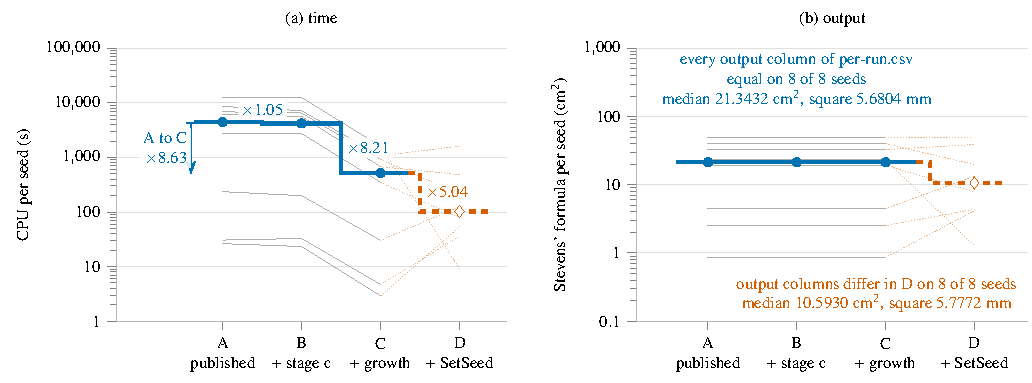
\includegraphics[width=\textwidth]{figures/c-f18-arms-steps}
\caption{Our changes to Stevens' pipeline added in turn, on the same PHerc.~0826 seeds (the arms of
Table~\ref{tab:arms}). (a) CPU time per seed, one grey line per seed, and the arm medians as steps,
each step labelled with its factor, the earlier median over the later. (b) Stevens' formula per seed,
the output of the same runs. Arms A, B and C are equal on every output column of
\texttt{per-run.csv} for every seed (patches, sheets, formula area, square, a2 share, crossing cells,
clean area), which is not a byte comparison of the sheets. Arm D, with the SetSeed reset, grows
something else and is drawn apart, dashed. Drawn by
\texttt{src/tools/c-f18-arms-steps.py} from \texttt{src/evidence/figures/c-f18-arms-steps.csv}.}
\label{fig:arms}
\end{figure*}

\begin{table*}[t]
\centering
\caption{Our changes to Stevens' pipeline on PHerc.~0826, added in turn. A: upstream as published.
B: plus the bad patch finder acceleration, the two corrections and the stage c commits. C: plus the
growth acceleration that passed the identity bar of Section~\ref{sec:growth}. D: plus the SetSeed velocity reset. An arm that did not finish in
time says so: «no run» means no seed of that arm completed by the cut off.}
\label{tab:arms}
\small
\setlength{\tabcolsep}{4pt}
\begin{tabular}{lrrrrrrrrr}
\toprule
arm & seeds & CPU (s) & wall (s) & sheets & formula (cm$^2$) & square (mm) & a2 share & crossing cells & deaths \\
\midrule
A & \ArmADone & \ArmACpu & \ArmAWall & \ArmASheets & \ArmAFormula & \ArmASquare & \ArmAAtwo & \ArmAVtwo & \ArmADeaths \\
B & \ArmBDone & \ArmBCpu & \ArmBWall & \ArmBSheets & \ArmBFormula & \ArmBSquare & \ArmBAtwo & \ArmBVtwo & \ArmBDeaths \\
C & \ArmCDone & \ArmCCpu & \ArmCWall & \ArmCSheets & \ArmCFormula & \ArmCSquare & \ArmCAtwo & \ArmCVtwo & \ArmCDeaths \\
D & \ArmDDone & \ArmDCpu & \ArmDWall & \ArmDSheets & \ArmDFormula & \ArmDSquare & \ArmDAtwo & \ArmDVtwo & \ArmDDeaths \\
\bottomrule
\end{tabular}
\end{table*}

\begin{table*}[t]
\centering
\caption{Neighbouring arms on the seeds both completed by the cut off: medians over exactly those
seeds, the earlier arm first. ``Not measurable'' means the two arms share no completed seed.}
\label{tab:paired}
\small
\begin{tabular}{lrrrrrrr}
\toprule
 & shared & \multicolumn{2}{c}{CPU (s)} & \multicolumn{2}{c}{formula (cm$^2$)} & \multicolumn{2}{c}{square (mm)} \\
pair & seeds & earlier & later & earlier & later & earlier & later \\
\midrule
A, B & \PairABShared & \PairABCpuOld & \PairABCpuNew & \PairABFormulaOld & \PairABFormulaNew & \PairABSquareOld & \PairABSquareNew \\
B, C & \PairBCShared & \PairBCCpuOld & \PairBCCpuNew & \PairBCFormulaOld & \PairBCFormulaNew & \PairBCSquareOld & \PairBCSquareNew \\
C, D & \PairCDShared & \PairCDCpuOld & \PairCDCpuNew & \PairCDFormulaOld & \PairCDFormulaNew & \PairCDSquareOld & \PairCDSquareNew \\
\bottomrule
\end{tabular}
\end{table*}
%% PENDING-END

The arms compare the two pipelines per seed, but a search pays per find, so we also compared them on squares found per
machine hour, counting every seed each search tried, with the formula declared before it was
computed.\footnote{\path{search-yield-0826/yield.csv}; the formula is in \path{src/prereg/search-yield-0826.md}.} A find is a
delivered sheet with a hole free square of \SourceThreshold{}~mm or more, or with a certified one. A seed counts once
however many of its sheets qualify, and machine hours are the summed seconds of the growths divided by the number
running at once. That number is a declared model, not a measurement: the declaration fixed it before any number at
\YieldOrigK{} growths at once for Stevens' pipeline and \YieldOursK{} for ours on the same machine,
and took each growth's wall time at that load to equal its wall time measured two at a time.\footnote{\path{src/prereg/search-yield-0826.md},
section on time.} Each rate is in proportion to that number, so a factor of \YieldOursK{} over \YieldOrigK{} in the
ratios below comes from the model. Table~\ref{tab:yield} gives every part of the charge.

Stevens' pipeline is charged arm~A's mean wall time and a full build for each seed the random waves delivered. That
makes \YieldOrigHours{} machine hours, in which it makes \YieldOrigFindsHf{} hole free finds and \YieldOrigFindsCert{}
certified ones, at rates of \YieldOrigRateHf{} and \YieldOrigRateCert{} per machine hour. These are upper bounds that
favour it: it is not charged for the seeds that die, and its finds are counted on our sheets, whose median best square
on the seeds of the arms is larger than arm~A's own. Ours is charged for every wave in the order it ran. The charge is
the seed rule steps, the ladder growths and their builds, arm~C's mean wall time for each delivered seed, and the chain's
own time for the seeds that grew and did not deliver. That comes to \YieldOursHours{} machine hours, in which ours makes
\YieldOursFindsHf{} hole free finds and \YieldOursFindsCert{} certified ones, at \YieldOursRateHf{} and
\YieldOursRateCert{} per machine hour. That is at least \YieldRatioHf{} times the original's for hole free squares, and
\YieldRatioCert{} times for certified ones. After the random waves alone ours stood at \YieldOursRandomRateHf{} and
\YieldOursRandomRateCert{}, so the waves drawn near earlier finds raised the finds per seed drawn but not per machine
hour. Charged instead with the chain's own delivery time, ours gives \YieldDeliveredRateHf{} and
\YieldDeliveredRateCert{} per machine hour.

\section{Limits}

The chain was still delivering when its files were copied, so they are frozen at its relaunch of \ChainFreezeTime{}.
Every count of Table~\ref{tab:waves} and Figure~\ref{fig:square} is of the seeds grown at \ChainGenCap{} generations
before it,\footnote{Column \texttt{chain\_as\_run} of \texttt{src/evidence/MANIFEST.csv}, one row per seed in
\texttt{derived/chain-as-run.csv}.} and the area numbers are over the smaller set of seeds their study froze. A
certificate means the checks passed and nothing more. The one lamina test sees two sheets only where they run parallel
at about one pitch over a declared area, so a group without conflicts is one lamina only as far as that test can see.
The checks do not see dark cells or a change of layer at a crack: a square of \RdSquare{}~mm that passes them has a
dark corner that runs through air. The adjudication of a crossing between traced surfaces leans on our own sheets, and where they agree equally with both
surfaces, both lose the cell. The fibre score looks only along the grid axes, so fibres at an angle to the grid score
lower, and it does not say what a surface that fails the bar is. The clean windows are found only on the sheets that
pass it, and the straightened sections are set against arithmetic, not against a measured null. The speed factors of
the growth are one seed on a quiet machine, and the rates per machine hour rest on a declared model of how many growths
run at once. Nothing here is a reading of ink on PHerc.~0826.

The checks have a blind spot for air. The house rule calls a cell dark when its grey is under \CutsDarkT{}, half the
median of the square of seed 2715. On this scan the grey of air lies above that value,\footnote{\path{src/prereg/cuts-2715.md}, the addition on the eye zooms at the crack.} so the checks can certify surface that
runs through air. We therefore cut the headline square across, on \CutsHead{} axial cuts declared before any number,
and looked for runs of at least \CutsVoidRun{} nodes off papyrus. There are \CutsHeadRuns{} such runs; the longest run is
\CutsHeadLongest{} nodes, \CutsHeadLongestMm{}~mm, at the left edge of the square, where by eye the surface leaves the
tip of a fold. The share of the square's cells with a grey of \CutsAirBar{} or less is \CutsAirHead{}, against
\CutsAirRd{} on the square of seed 2715 and \CutsAirCorner{} in its dark corner.\footnote{\path{headline-cuts.csv},
\path{headline-eye.csv}, \path{headline-air.csv} and \path{air-reference.csv} of study \texttt{cuts-2715}.}

\section{Open questions}

Can a label free statistic see ink that the labels show? On PHerc.~0139 our sheets carry the labelled ink to the
released model, yet the statistic we used on PHerc.~0826 says no on every row of that known ink. Until a statistic says
yes where the labels do, reads of PHerc.~0826 remain \PcInkReading{}. A statistic that passes on the labelled rows of
PHerc.~0139, run the same way, would settle whether the certified square can be read.

Do the checks hold on surfaces that are not ours? They judge a sheet in the grid that Stevens' flattening writes, and
the crossing test compares a sheet with the other sheets this pipeline delivered. The certified square shows they can
judge a surface grown by the organisers' tracer when our sheets are near it. A tool that reads tifxyz, judges one
segment on its own and takes its fibre bar from public segments would say whether they hold on the organisers' own
segments.

Is the fibre bar measuring papyrus or the angle of the grid? The bar is a fraction of the score of one of our own
sheets, and the score looks only along the grid axes, while the windows' grids lie \WinAngleMin{} to \WinAngleMax{}
degrees from the scan's height. Scoring the same pieces on the resampled grid of Figure~\ref{fig:windows} would say how
many of the \FibreTopFailCount{} largest certified pieces fail for their angle rather than their surface.

Does the adjudication choose the right surface where our sheets are absent? A crossing decided by our sheets inherits
their errors, and where they agree equally with both surfaces both lose the cell. A reference that does not come from
this pipeline, such as a labelled segment crossing the same region, would say whether the kept surface is the one on
papyrus.

\section{Conclusion}

On PHerc.~0826 a loop with no person in it runs Stevens' pipeline with corrections that change its sheets, and a set of
automatic checks decides which of its surfaces to keep. Without the corrections, our changes make the pipeline
\ArmFactorAC{} times faster per seed with every measured output equal. The checks certify a square of
\RcOneSquare{}~mm on a surface grown by the organisers' tracer from a start our search chose, and they reject the
largest pieces of our own sheets, which fail the fibre test. For someone using the code, the change is that a surface
is kept or rejected by stated checks rather than by eye, whichever program grew it.

What the certificate does not establish is that the square can be read. The positive control on PHerc.~0139 shows that
our sheets carry labelled ink to the released model, and it also shows that our label free statistic cannot yet say so
on a scroll without labels.
